\documentclass[a4paper]{article}
\addtolength{\hoffset}{-2.25cm}
\addtolength{\textwidth}{4.5cm}
\addtolength{\voffset}{-3.25cm}
\addtolength{\textheight}{5cm}
\setlength{\parindent}{15pt}

\usepackage[unicode=true, colorlinks=false, hidelinks]{hyperref}
\usepackage[utf8]{inputenc}
\usepackage[english, russian]{babel}
\usepackage{mathtext}
\usepackage[T2A, TS1]{fontenc}
\usepackage{microtype} % Slightly tweak font spacing for aesthetics
\usepackage{amsthm, amssymb, amsmath, amsfonts, nccmath}
\usepackage{nicefrac}
\usepackage{epstopdf}
\usepackage[export]{adjustbox}
\usepackage{float} % Improved interface for floating objects
\usepackage{graphicx, multicol} % Enhanced support for graphics
\usepackage{pdfrender,xcolor}
\usepackage{breqn}
\usepackage{mathtools}
\usepackage{titling}
\usepackage{bm}
\usepackage{centernot}
\usepackage[cal=boondoxo,calscaled=.96]{mathalpha}
\usepackage{marvosym, wasysym} % More symbols
\usepackage{rotating} % Rotation tools
\usepackage{censor} % Facilities for controlling restricted text
\usepackage{indentfirst}
\usepackage{svg}

\DeclareMathOperator{\rad}{rad}
\DeclareMathOperator{\imid}{mid}
\DeclareMathOperator{\sign}{sign}
\newcommand{\mbb}[1]{\mathbb{#1}}
\newcommand{\mbf}[1]{\mathbf{#1}}

\usepackage{array}
\newcolumntype{C}[1]{>{\centering\let\newline\\\arraybackslash\hspace{0pt}}m{#1}}

\usepackage{fancyhdr}
\pagestyle{fancy}
\fancyhead{}\renewcommand{\headrulewidth}{0pt}
\fancyfoot[L]{}
\fancyhead{}
\fancyfoot{}
\fancyfoot[R]{\thepage}
\begin{document}
\large
\begin{center}
    Санкт-Петербургский политехнический университет\\
    Высшая школа прикладной математики и\\вычислительной физики,\\ 
    Физико-механический институт\\
    \vspace{3em}
    Направление подготовки\\
    01.03.02 «Прикладная математика и информатика»\\
    \vspace{10em}
    \Large
    Отчет по лабораторной работе №3 \\
    по дисциплине «Интервальный анализ»
    \vspace{19em}
    \large
\end{center}
Выполнил студент гр. 5030102/80201\\
Кирпиченко С. Р.\\
Руководитель\\
Баженов А. Н.
\vspace{10em}
\begin{center}
    Санкт-Петербург\\
    2021
\end{center}
\thispagestyle{empty}
\newpage
\tableofcontents
\addtocontents{toc}{~\hfill\textbf{Страница}\par}
\newpage
\listoffigures
\addtocontents{lof}{~\hfill\textbf{Страница}\par}
\newpage
\section{Постановка задачи}
Дана ИСЛАУ 
\begin{equation}\label{islau}
    \begin{cases}
    [0,\:2]\cdot x_1+[1,\:3]\cdot x_2=[3,\:7]\\
    x_1 - [2,\:4]\cdot x_2=0\\
    [1,\:3]\cdot x_1=[5,\:7]\\
    \end{cases}
\end{equation}
Для нее необходимо провести вычисления и привести иллюстрации:
\begin{itemize}
    \item Максимума распознающего функционала
    \item Достижения разрешимости ИСЛАУ за счет коррекции правой части
    \item Достижения разрешимости ИСЛАУ за счет коррекции матрицы
    \item Оценок вариабельности решения
    \item Управления положением максимума распознающего функционала за счет коррекции матрицы ИСЛАУ в целом
    \item Управления положением максимума распознающего функционала за счет коррекции матрицы ИСЛАУ построчно
\end{itemize}

\section{Теория}
\subsection{Распознающий функционал}
Распознающим называется функционал 
\begin{equation*}
    \mathrm{Tol}(x)=\mathrm{Tol}(x,\mbf{A},\mbf{b})=\min_{1\leq i\leq m}\left\{\rad{\mbf{b}_i}-\left|\imid{\mbf{b}_i}-\sum_{j=1}^n \mbf{a}_{ij}x_j\right|\right\}
\end{equation*}
\begin{equation*}
    x\in\Xi_{\mathrm{tol}}\Leftrightarrow\mathrm{Tol}(x)\geq0
\end{equation*}
$\mathrm{Tol}(x)$ - ограничен, вогнут. Он всегда достигает конечного максимума на $\mbb{R}^n$. Таким образом, найдя максимум данного функционала, можно судить о пустоте допускового множества решений ИСЛАУ. Если $\max\limits_{x\in\mbb{R}^n}\mathrm{Tol}(x)\geq0$, то допусковое множество не пусто. В противном случае $\Xi_{\mathrm{tol}}=\varnothing$. Обратные утверждения также верны.
\subsection{Достижение разрешимости ИСЛАУ за счет коррекции правой части}
Общая схема метода заключается в добавлении к каждой компоненте правой части ИСЛАУ величины $K\cdot\nu_i\cdot[-1,\:1]$, где $i$ - номер компоненты, $\nu_i$ - вес, задающий относительное расширение $i$-й компоненты, $K$ - общий коэффициент расширения вектора $\mbf{b}$. В данной работе используются значение $\nu_i=1\;\forall i=\overline{1,3}$. Подобрав $K$ таким образом, чтобы выполнялось $ K +\max\limits_{x\in\mbb{R}^n}\mathrm{Tol}(x)\geq0$, получим разрешимую систему с непустым допусковым множеством.
\subsection{Достижение разрешимости ИСЛАУ за счет коррекции матрицы}
Общая схема метода заключается в модификации исходной матрицы ИСЛАУ. Производим замену $\mbf{A}$ на $\mbf{A}\ominus K\cdot N\cdot\mbf{E}$ где $ N=\{\nu_i\}$ - матрица весов, $K$ - общий коэффициент сужения $\mbf{A}$, $\mbf{E}$ состоит из $[-e_{ij},\:e_{ij}]$. При выполнении процедуры необходимо следить за тем, чтобы мы оставались в рамках $\mbb{IR}$. 

При выполнении задания достижения разрешимости рекомендуется выполнять корректировку пропорционально координатам точки, в которой достигается максимум распознающего функционала. 

При выполнении задания управления положением максимума распознающего функционала в случае коррекции матрицы в целом $N$ - единичная матрица, в случае построчной - $ N=\mathrm{diag}\{\nu_i\}$. 
\subsection{Оценки вариабельности решения}
Для оценки вариабельности решений предлагается использовать абсолютную и относительную оценки:
$$\mathrm{ive}(\mbf{A},\mbf{b})=\min\limits_{A\in\mbf{A}}\mathrm{cond}\:A\cdot||\mathrm{argmax}\:\mathrm{Tol}(x)||\frac{\max\limits_{x\in\mbb{R}^n}\mathrm{Tol}(x)}{||\mbf{b}||}$$
$$\mathrm{rve}(\mbf{A},\mbf{b})=\min\limits_{A\in\mbf{A}}\mathrm{cond}\:A\cdot\max\limits_{x\in\mbb{R}^n}\mathrm{Tol}(x)$$
\section{Реализация}
Для осуществления вычислений и визуализации результатов использовалась среда Matlab с библиотекой интервальной арифметики IntLab. Также использовалась функция tolsolvty для нахождения максимума распознающего функционала. Минимальное число обусловленности вычислялось стохастическим методом. 
\section{Результаты}
\subsection{Достижение разрешимости ИСЛАУ}
Изначальная ИСЛАУ имеет пустое допусковое множество, так как максимум распознающего функционала в точке $(3,1)$ равен -2. Этот максимум здесь и далее обозначен звездочкой.
\begin{figure}[H]
    \centering
    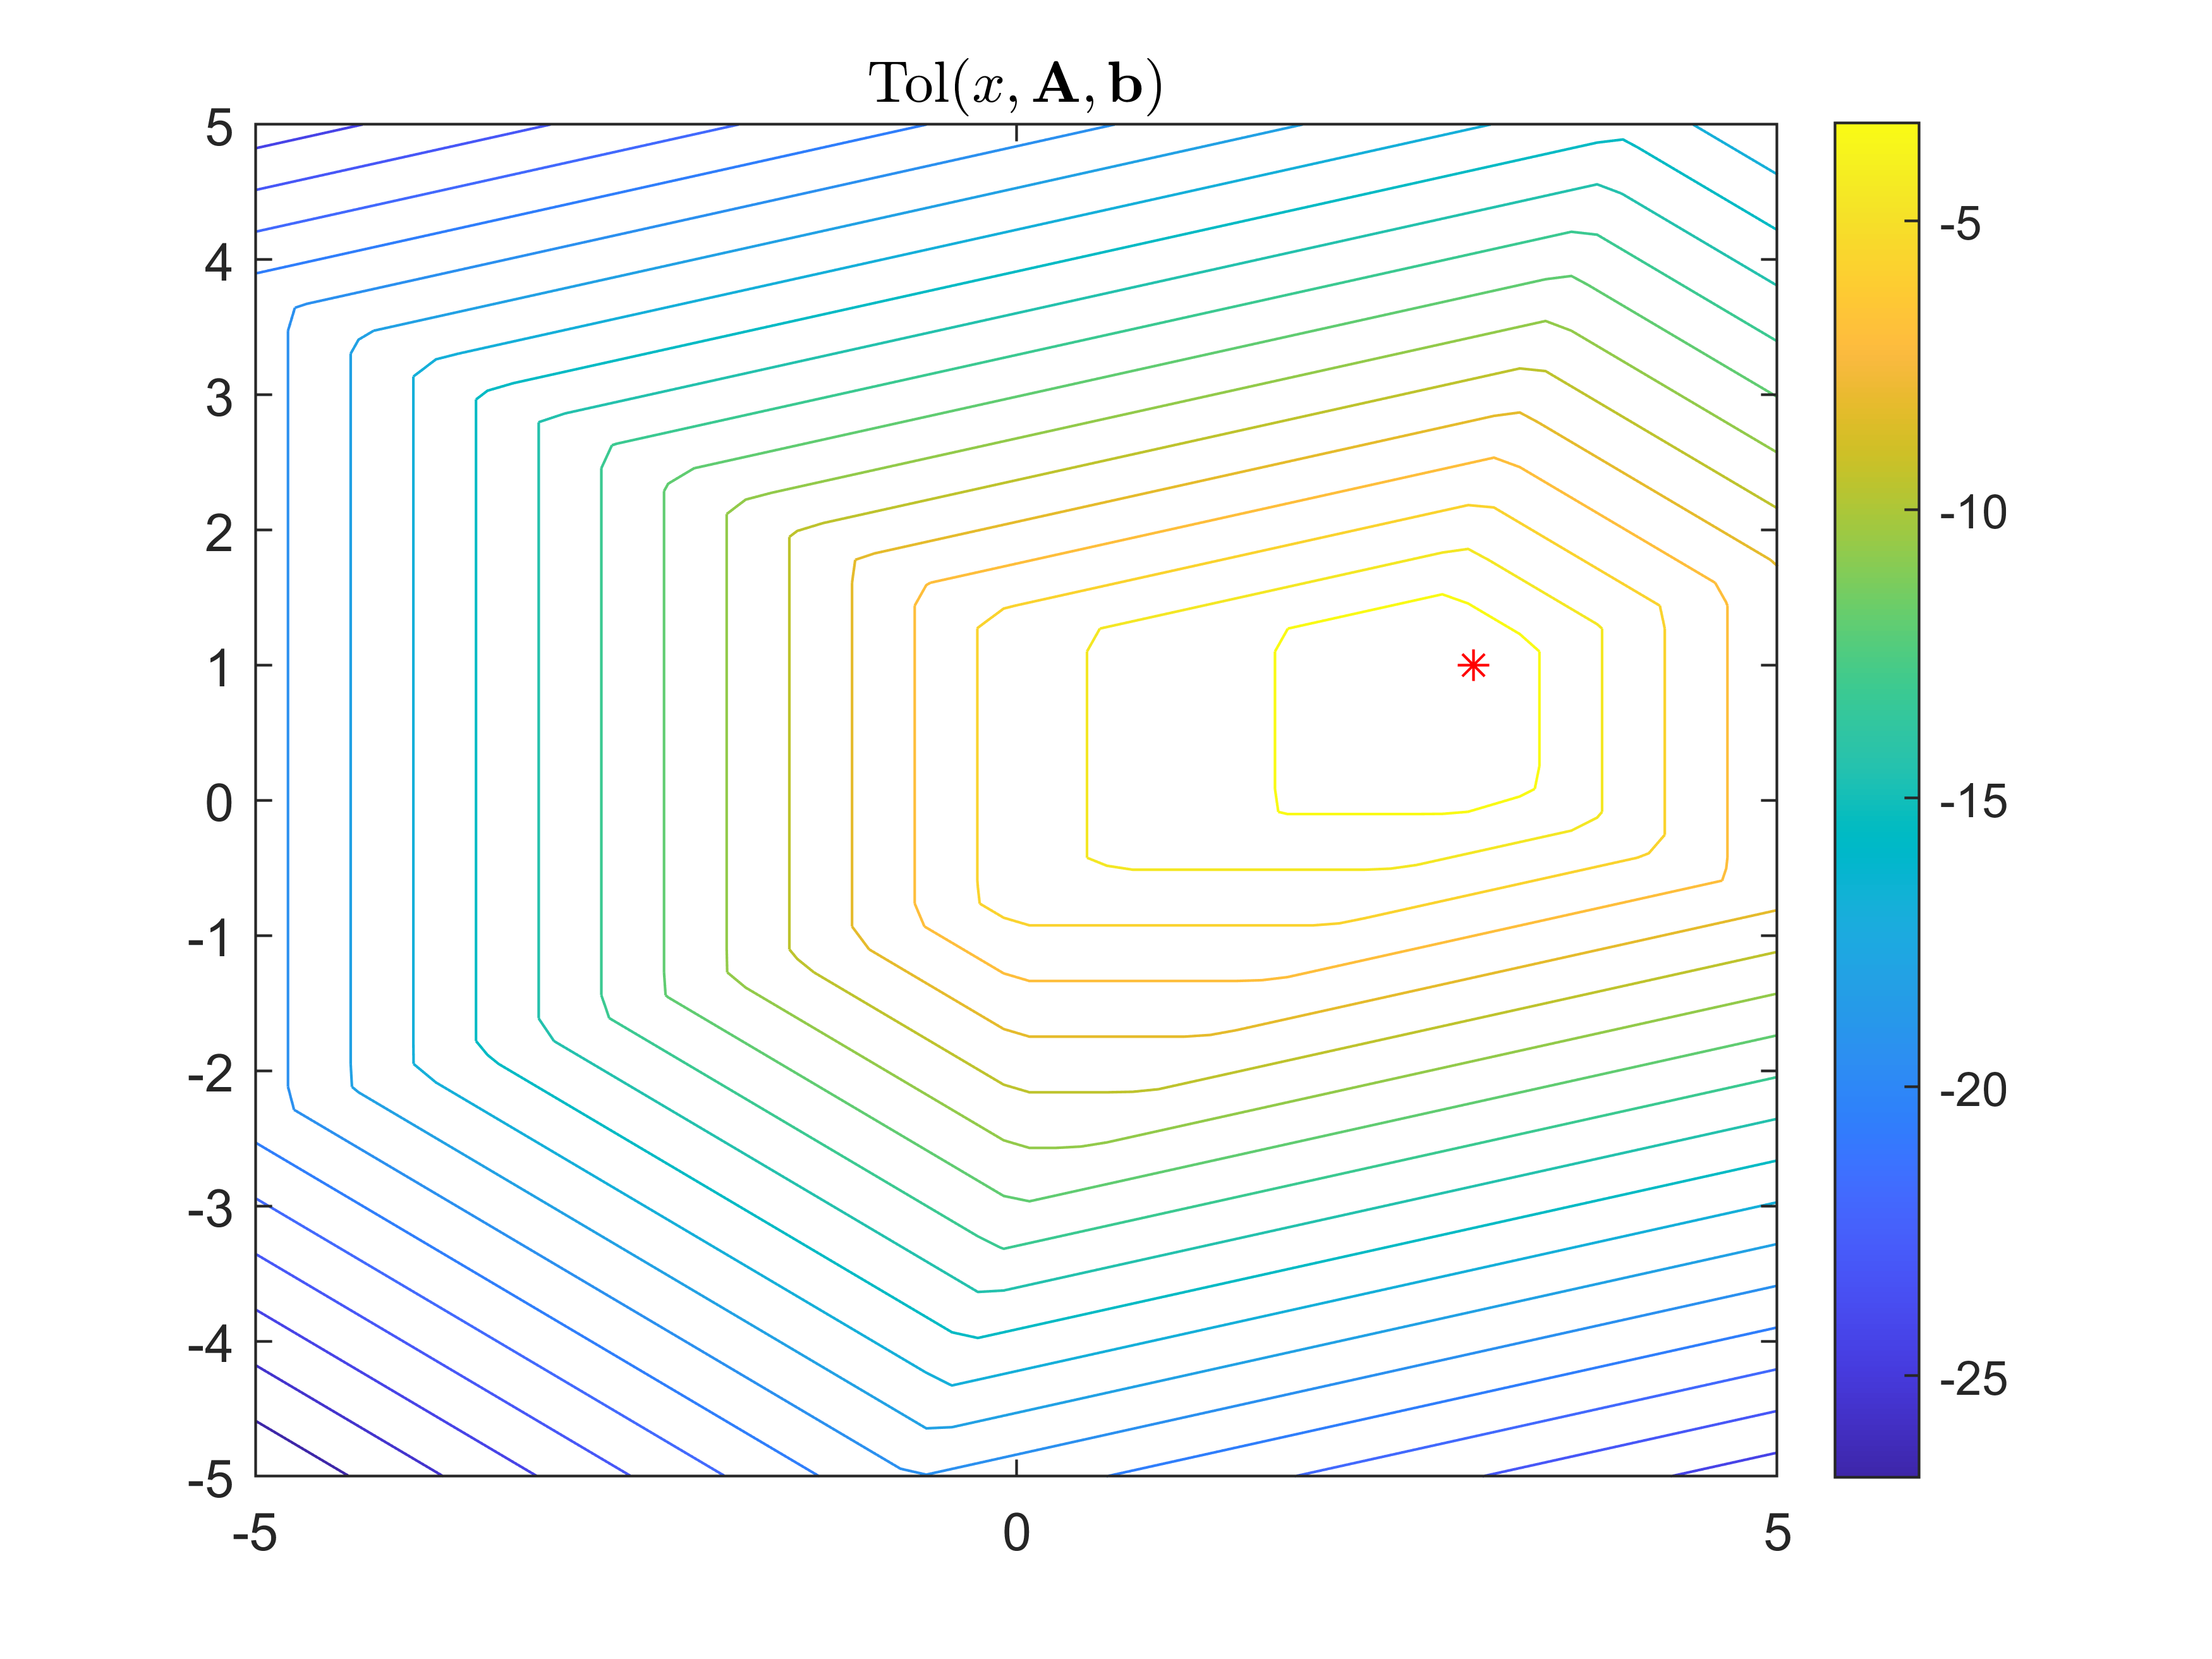
\includegraphics[width=15cm]{img/maxtol.png}
    \caption{График $\mathrm{Tol}(x,\mbf{A},\mbf{b})$}
    \label{fig:origtol}
\end{figure}
Для достижения разрешимости правая часть системы была заменена по описанной схеме с коэффициентом расширения  $K=1.5\cdot|\max\limits_{x\in\mbb{R}^n}\mathrm{Tol}(x)|=3$. $\hat{\mbf{b}}=\left(\begin{smallmatrix}
    [0,\:10]\\ [-3,\:3]\\ [2,\:10]
    \end{smallmatrix}\right)$. После коррекции максимум распознающего функционала стал равен $1$ в точке $(3,1)$.
\begin{figure}[H]
    \centering
    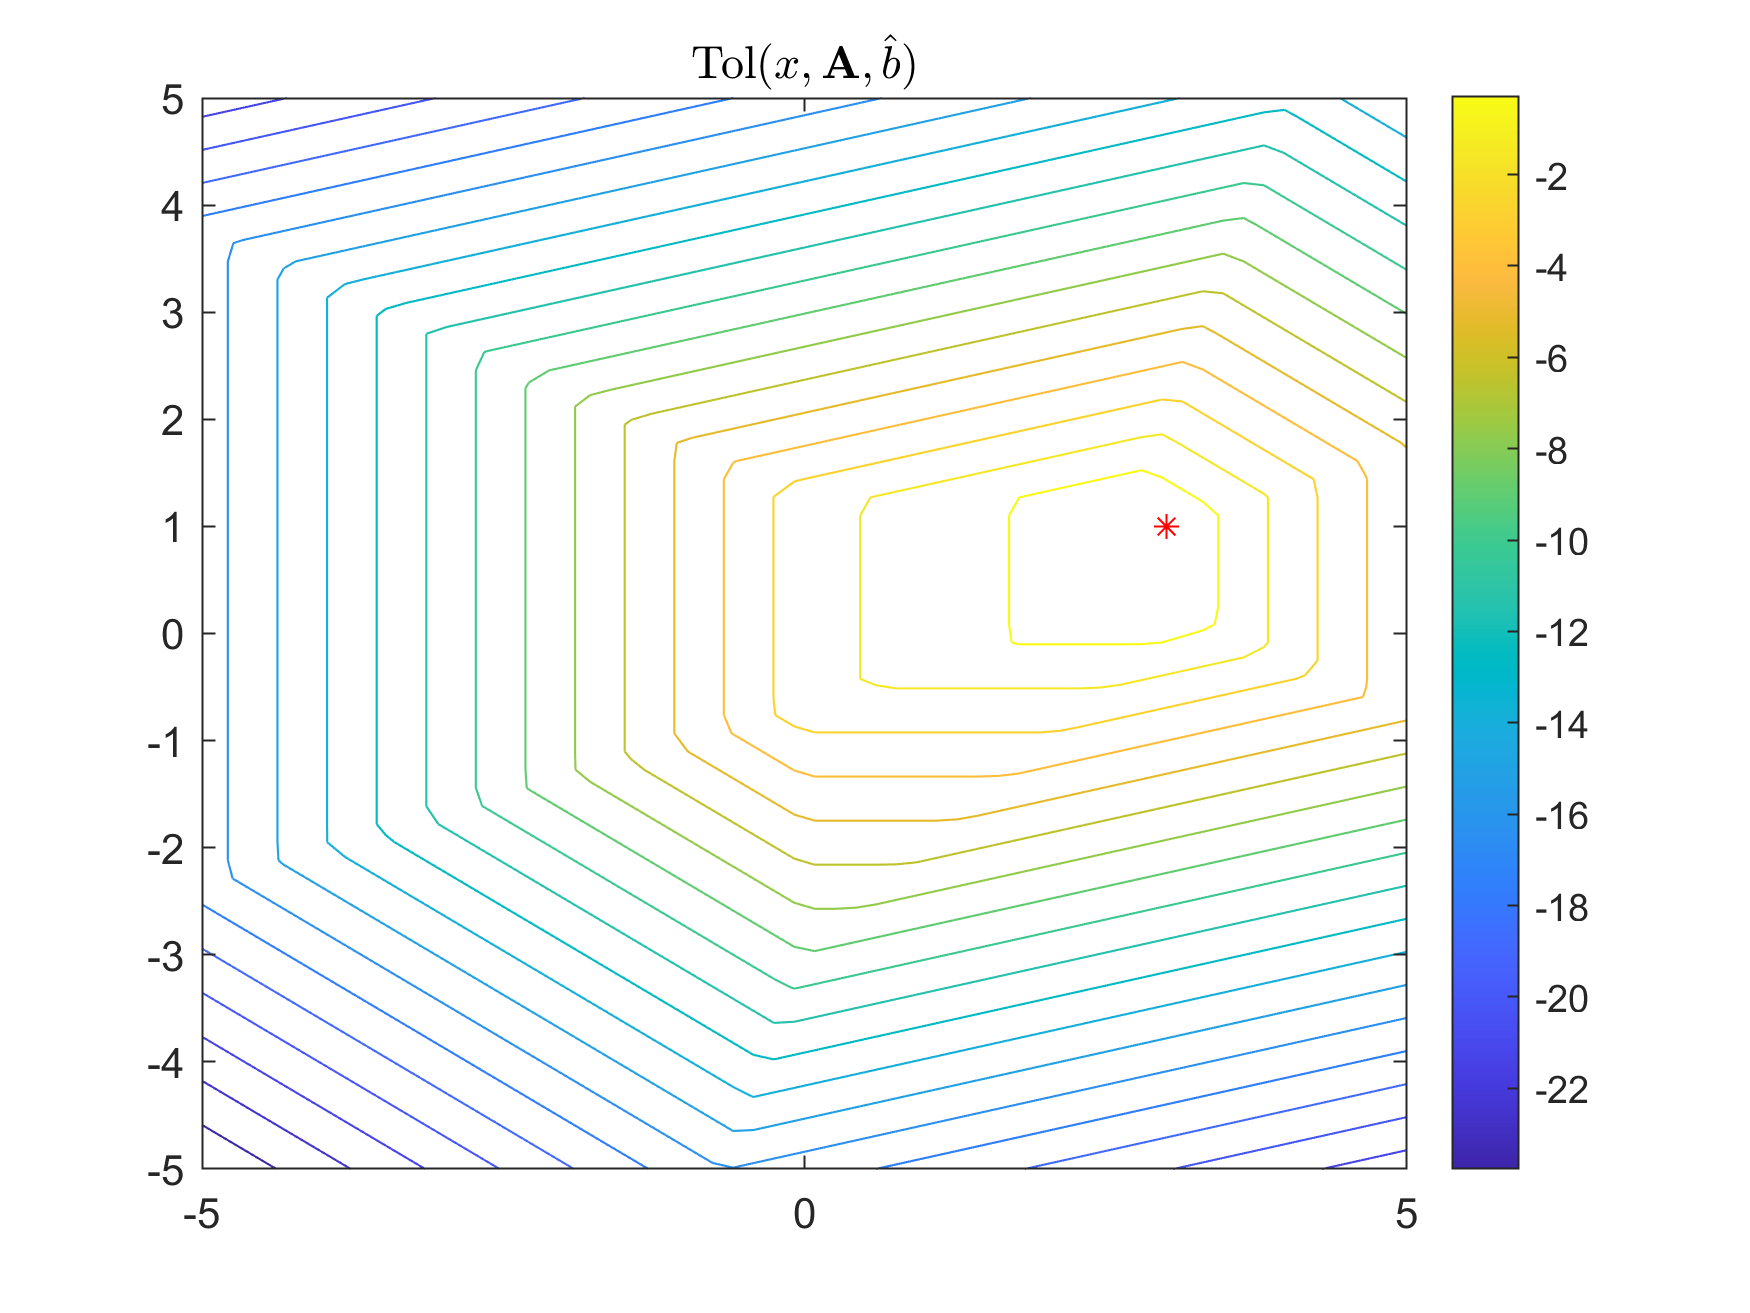
\includegraphics[width=12cm]{img/maxtol b.png}
    \caption{График $\mathrm{Tol}(x,\mbf{A}, \hat{\mbf{b}})$ для ИСЛАУ с правленной правой частью}
    \label{fig:btol}
\end{figure}
Допусковое множество решений стало непустым, оно отмечено на графике пунктиром. $\mathrm{ive}\:(\mbf{A}, \hat{\mbf{b}})\approx0.24,\;\mathrm{rve}\:(\mbf{A}, \hat{\mbf{b}})\approx1.1$. На графике изображены квадратные брусы с центром в точке максимума $\mathrm{Tol}\:(x)$ и радиусом $\mathrm{ive}$ и $\mathrm{rve}$.
\begin{figure}[H]
    \centering
    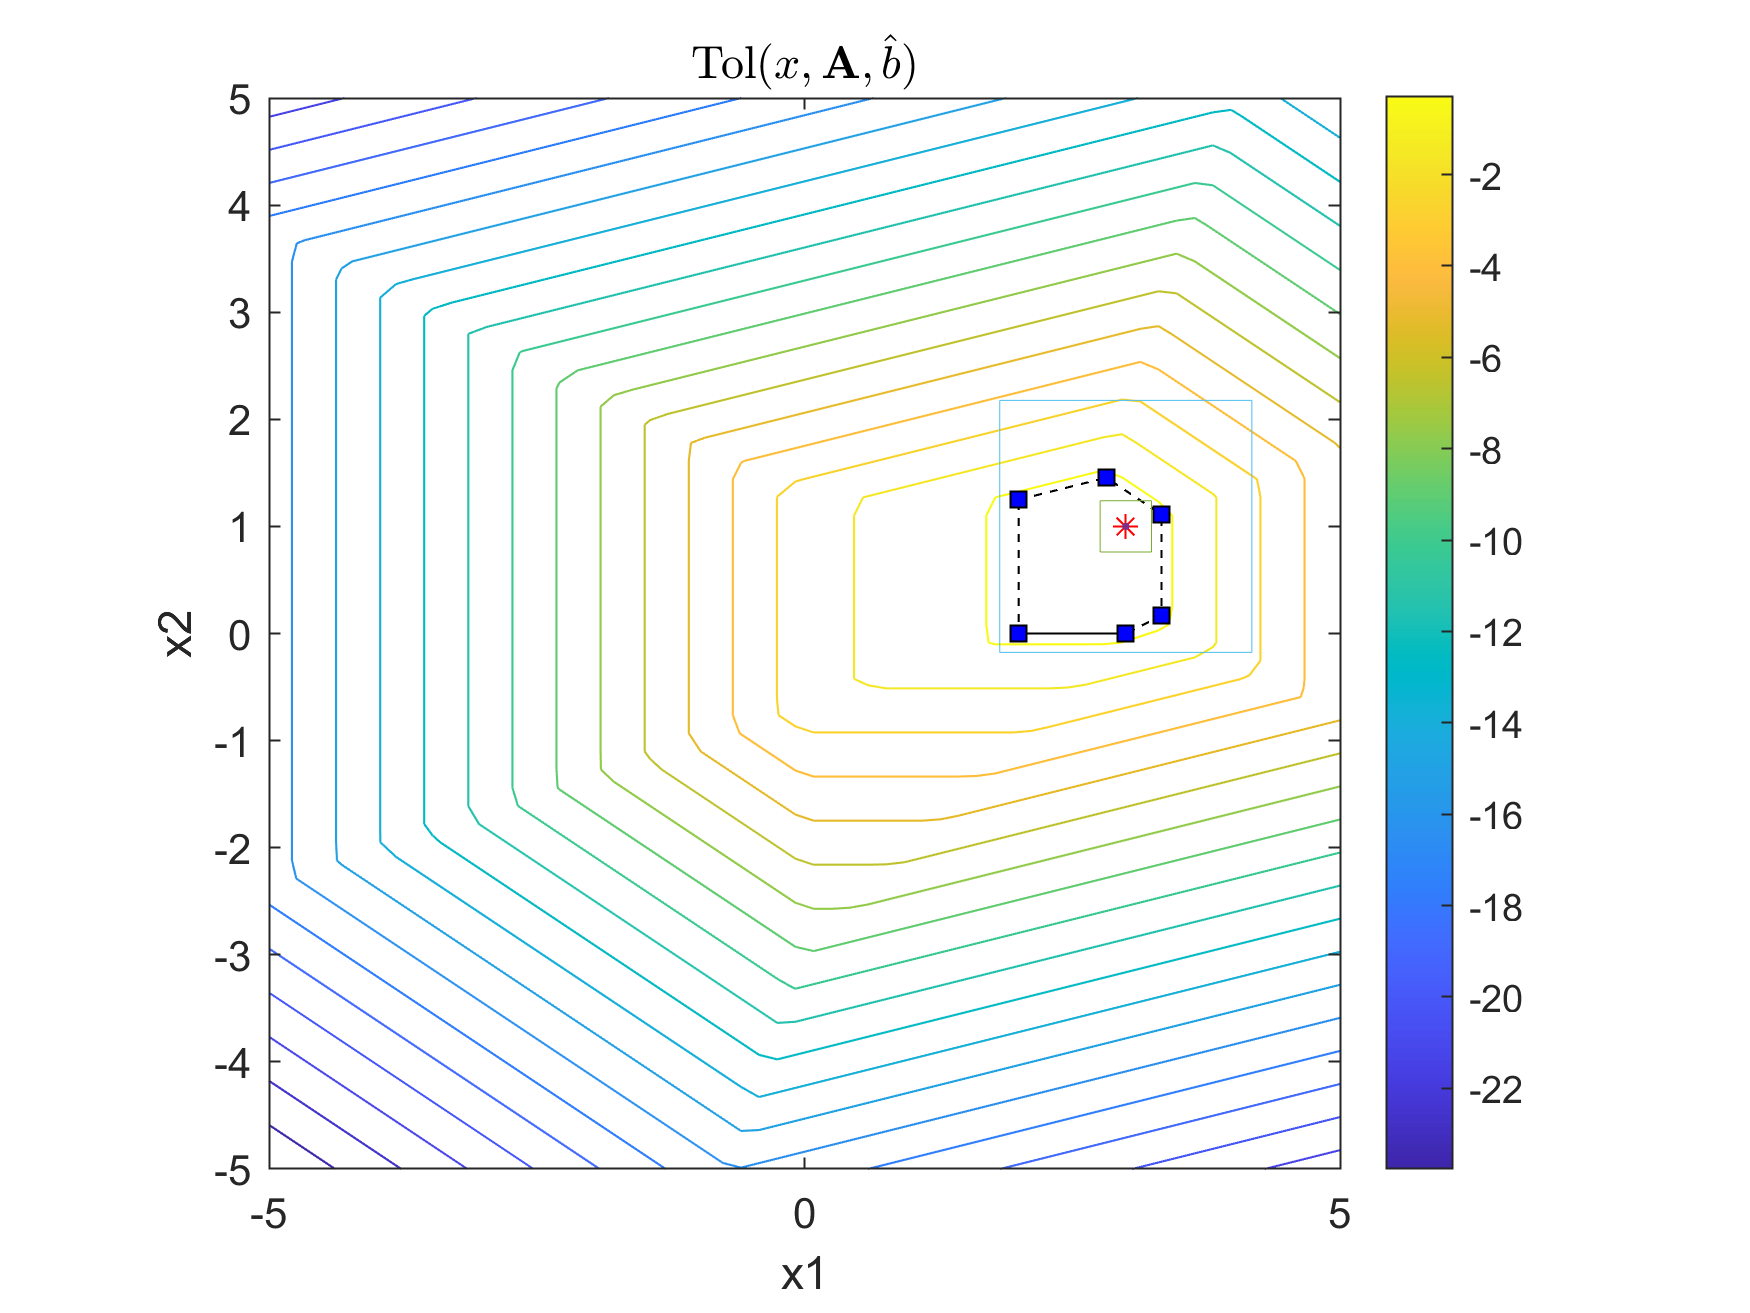
\includegraphics[width=12cm]{img/ive rve b.png}
    \caption{График $\Xi_{\mathrm{tol}}$ и оценки вариабельности для ИСЛАУ с правленной правой частью}
    \label{fig:biverve}
\end{figure}
При проведении коррекции матрицы для достижения разрешимости ИСЛАУ были выбраны следующие значения:
$$
\mbf{E}=\begin{pmatrix}
[-0.75,\:0.75]&[-1,\:1]\\
0&[-1,\:1]\\
[-0.75,\:0.75]&0
\end{pmatrix}\;
\hat{\mbf{A}}=\begin{pmatrix}
[0.75,\:1.25]&2\\
1&-3\\
[1.75,\:2.25]&0
\end{pmatrix}
$$
После коррекции максимум распознающего функционала стал равен $0$ в точке $(3,1)$.
\begin{figure}[H]
    \centering
    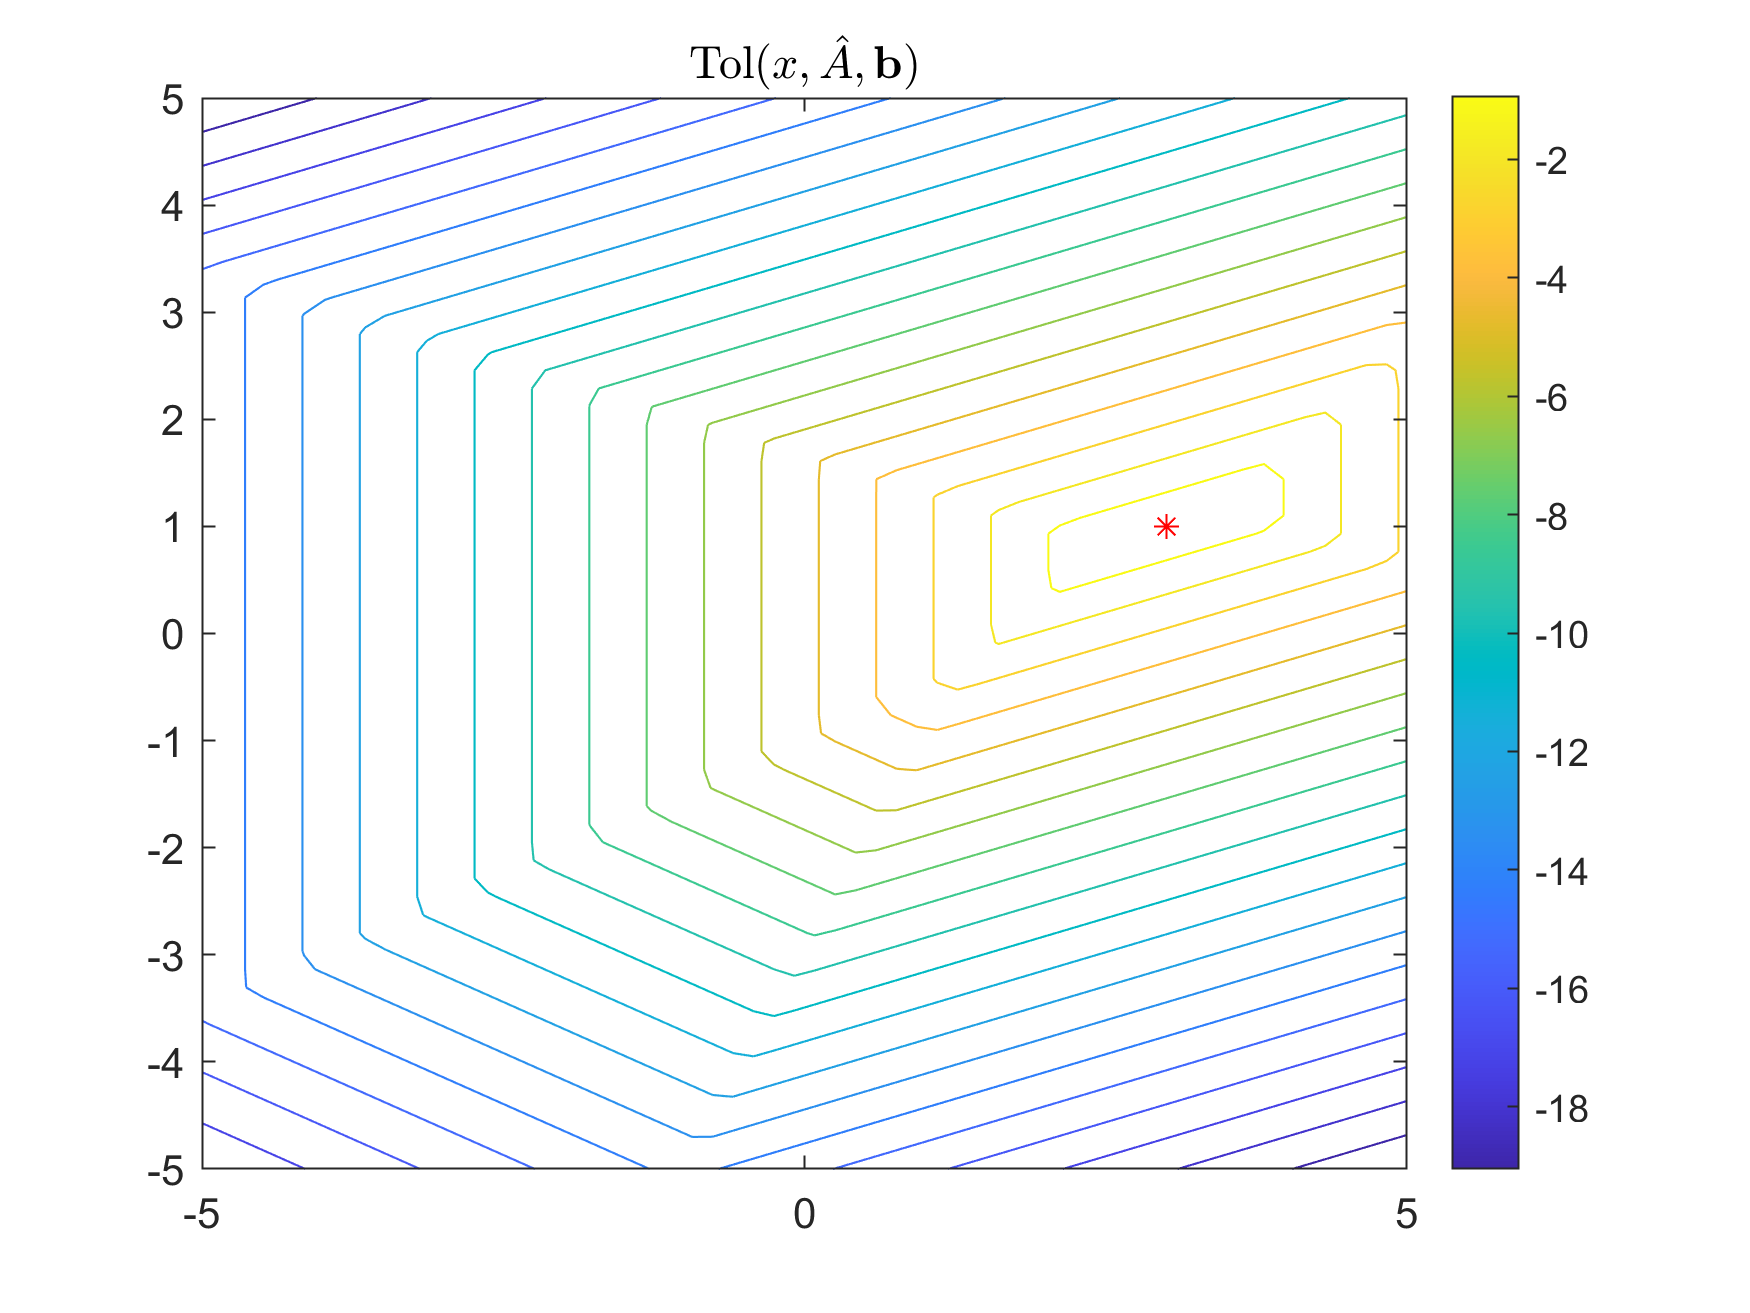
\includegraphics[width=11cm]{img/maxtol a.png}
    \caption{График $\mathrm{Tol}(x,\hat{\mbf{A}}, \mbf{b})$ для ИСЛАУ с правленной матрицей}
    \label{fig:atol}
\end{figure}
Допусковое множество решений стало непустым, отрезок отмечен на графике пунктиром. $\mathrm{ive}\:(\hat{\mbf{A}}, \mbf{b})=\mathrm{rve}\:(\hat{\mbf{A}}, \mbf{b})=0$. 
\begin{figure}[H]
    \centering
    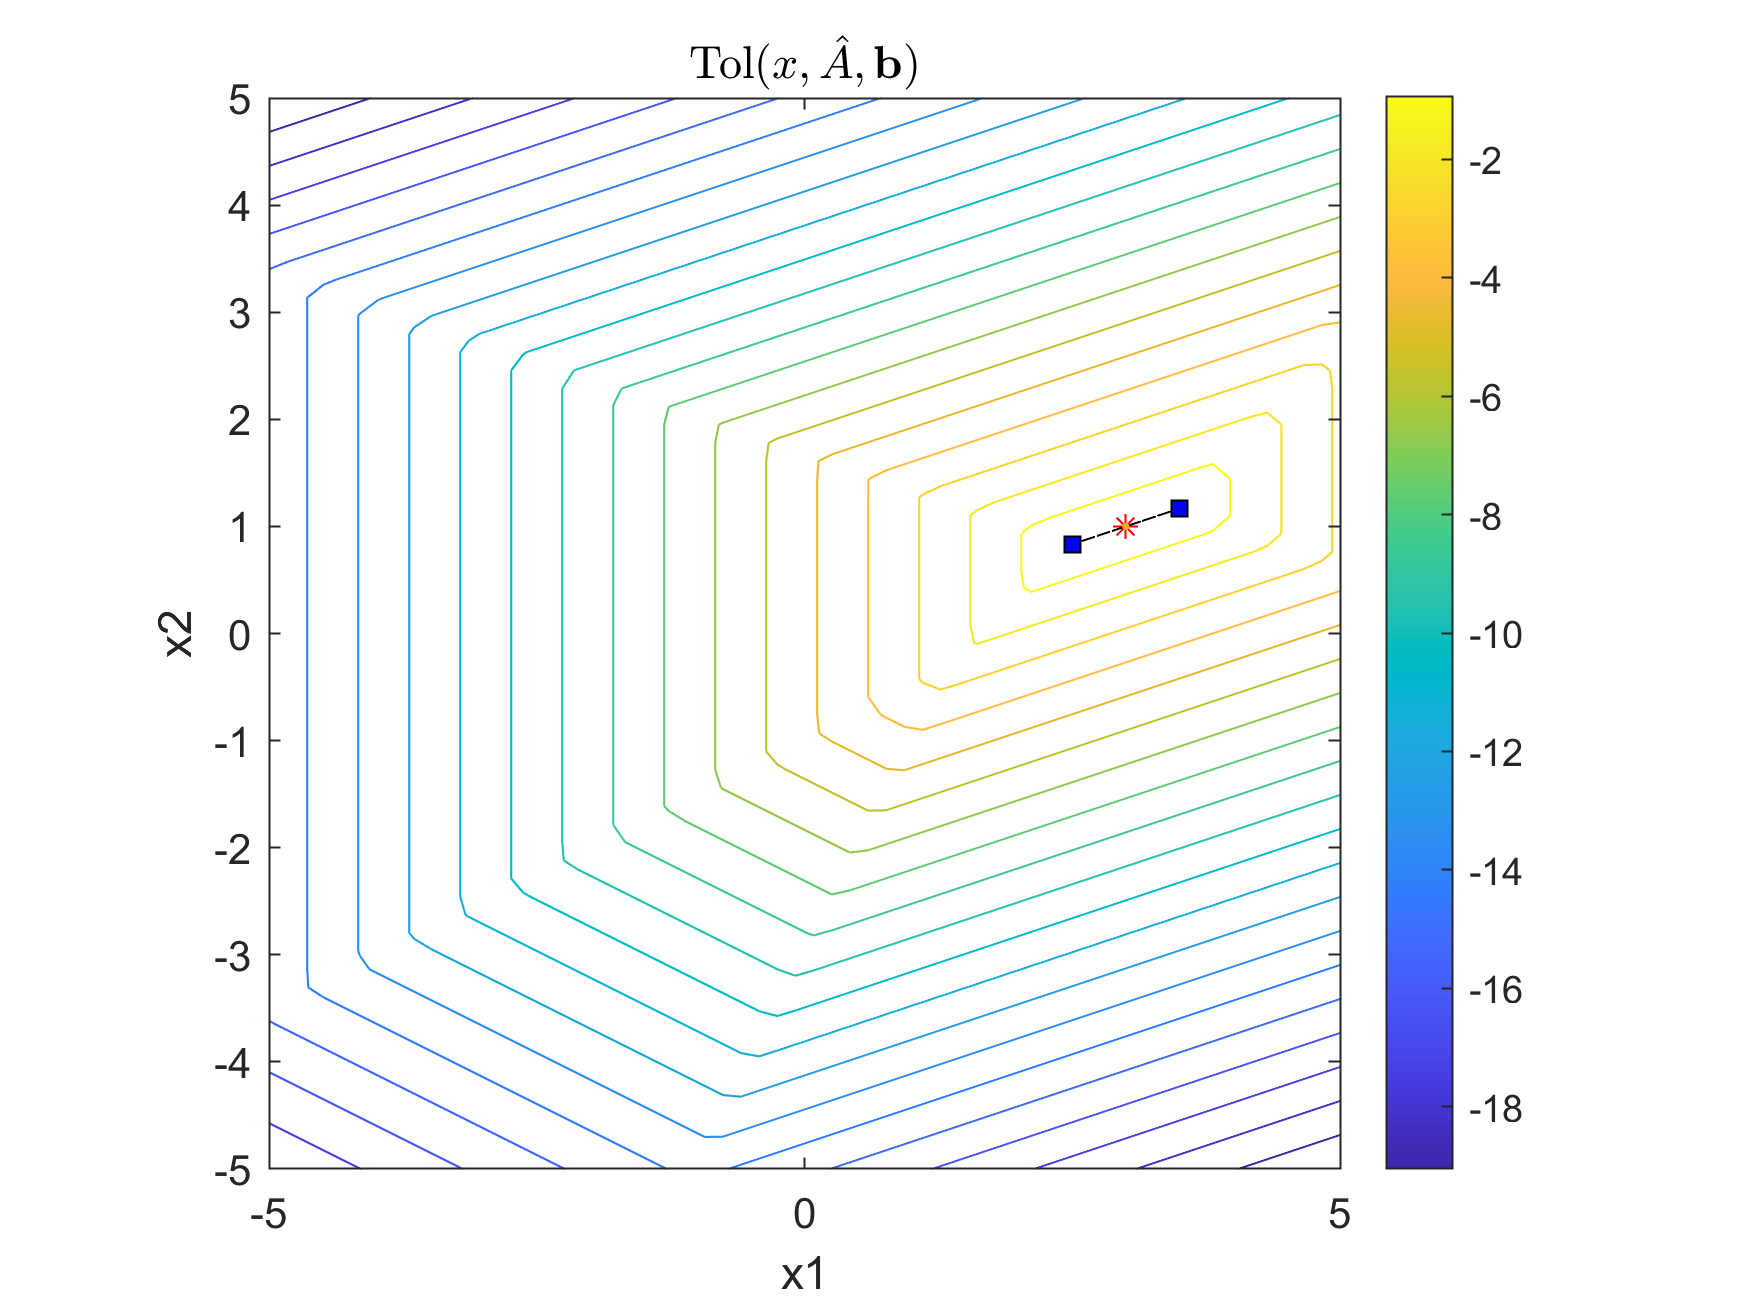
\includegraphics[width=11.5cm]{img/ive rve a.png}
    \caption{График $\Xi_{\mathrm{tol}}$ для ИСЛАУ с правленной матрицей}
    \label{fig:aiverve}
\end{figure}
\subsection{Управление положением максимума распознающего функционала}
Отметим на графике распознающего функционала прямые, образованные СЛАУ $\imid{(\mbf{A})}x=\imid{\mbf{b}}$. Красной прямой соответствует первая строка, зеленой - вторая, синей - третья.
\begin{figure}[H]
    \centering
    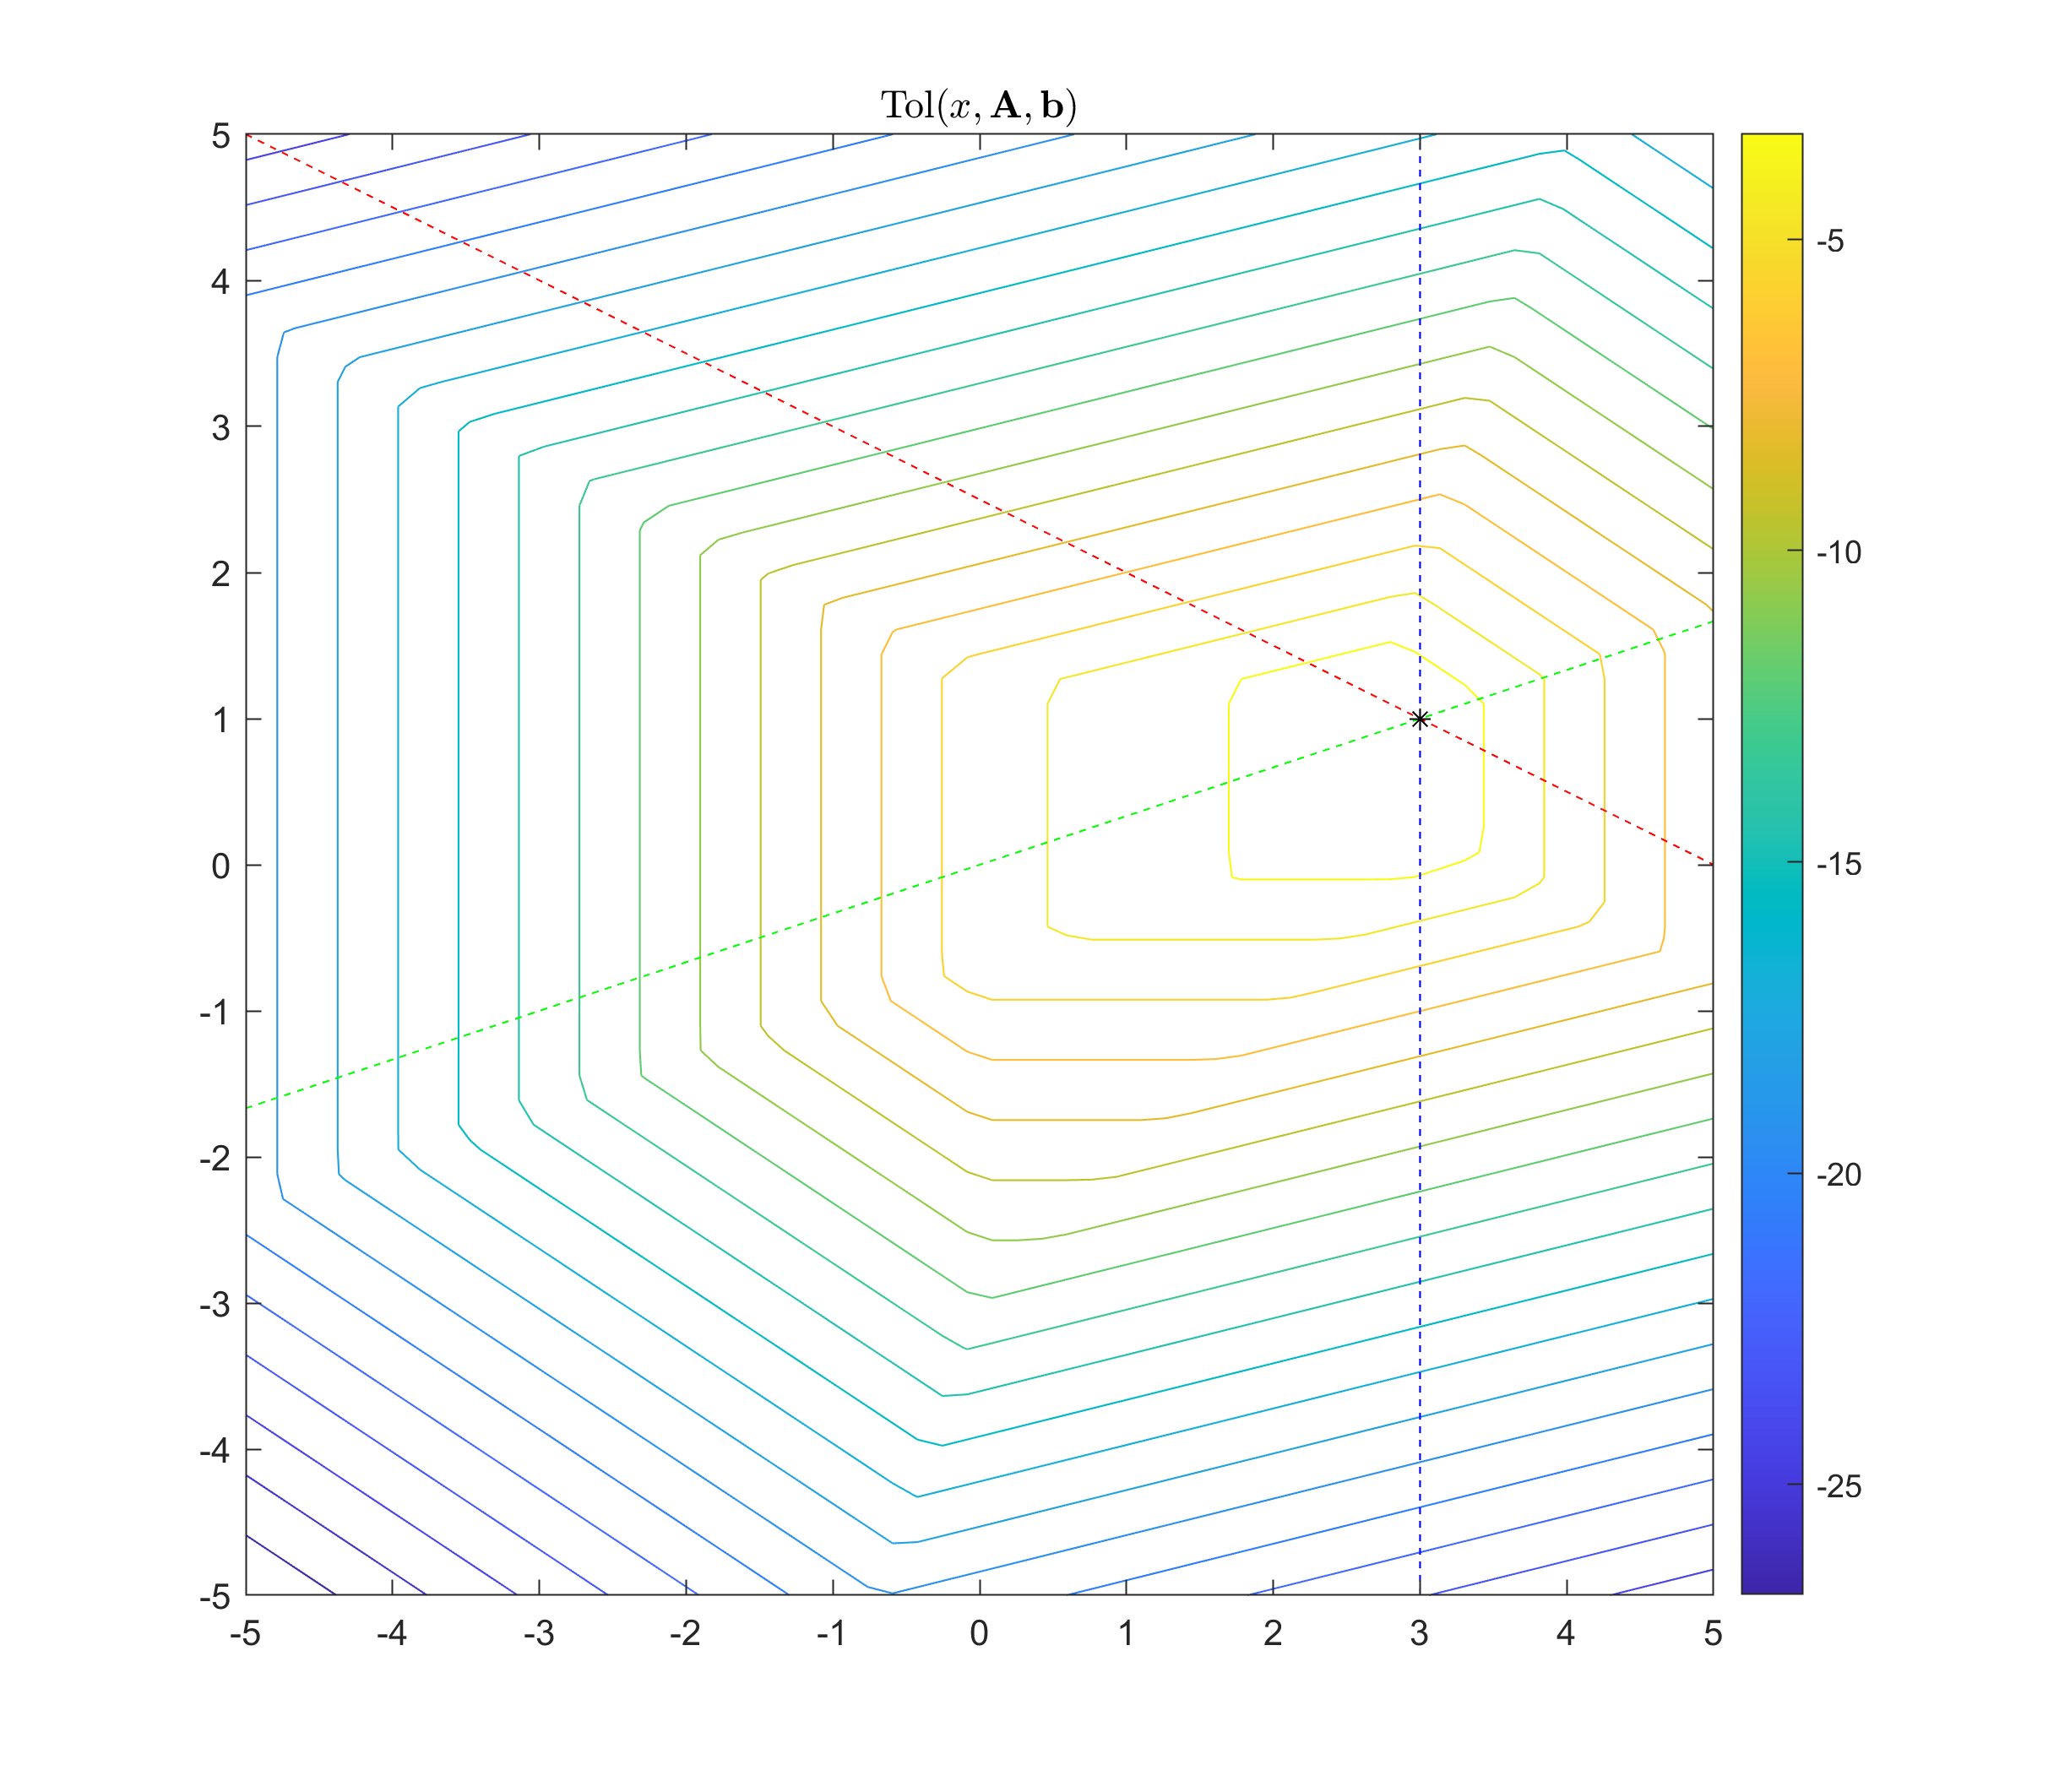
\includegraphics[width=15cm]{img/lines0.png}
    \caption{График $\mathrm{Tol}(x,\mbf{A},\mbf{b})$ с прямыми уравнений $\imid{(\mbf{A})}x=\imid{\mbf{b}}$}
    \label{fig:lines0}
\end{figure}
Результат корректировки матрицы в целом:
\begin{equation*}
    \check{\mbf{A}}=\begin{pmatrix}
    [0.5,\:1.5]&[1.5,\:2.5]\\
    1&[-3.5,\:-2.5]\\
    [1.5,\:2.5]&0
    \end{pmatrix},\;\mathrm{arg}\max\mathrm{Tol}(x,\check{\mbf{A}}, \mbf{b})=(3,1)
\end{equation*}
\begin{figure}[H]
    \centering
    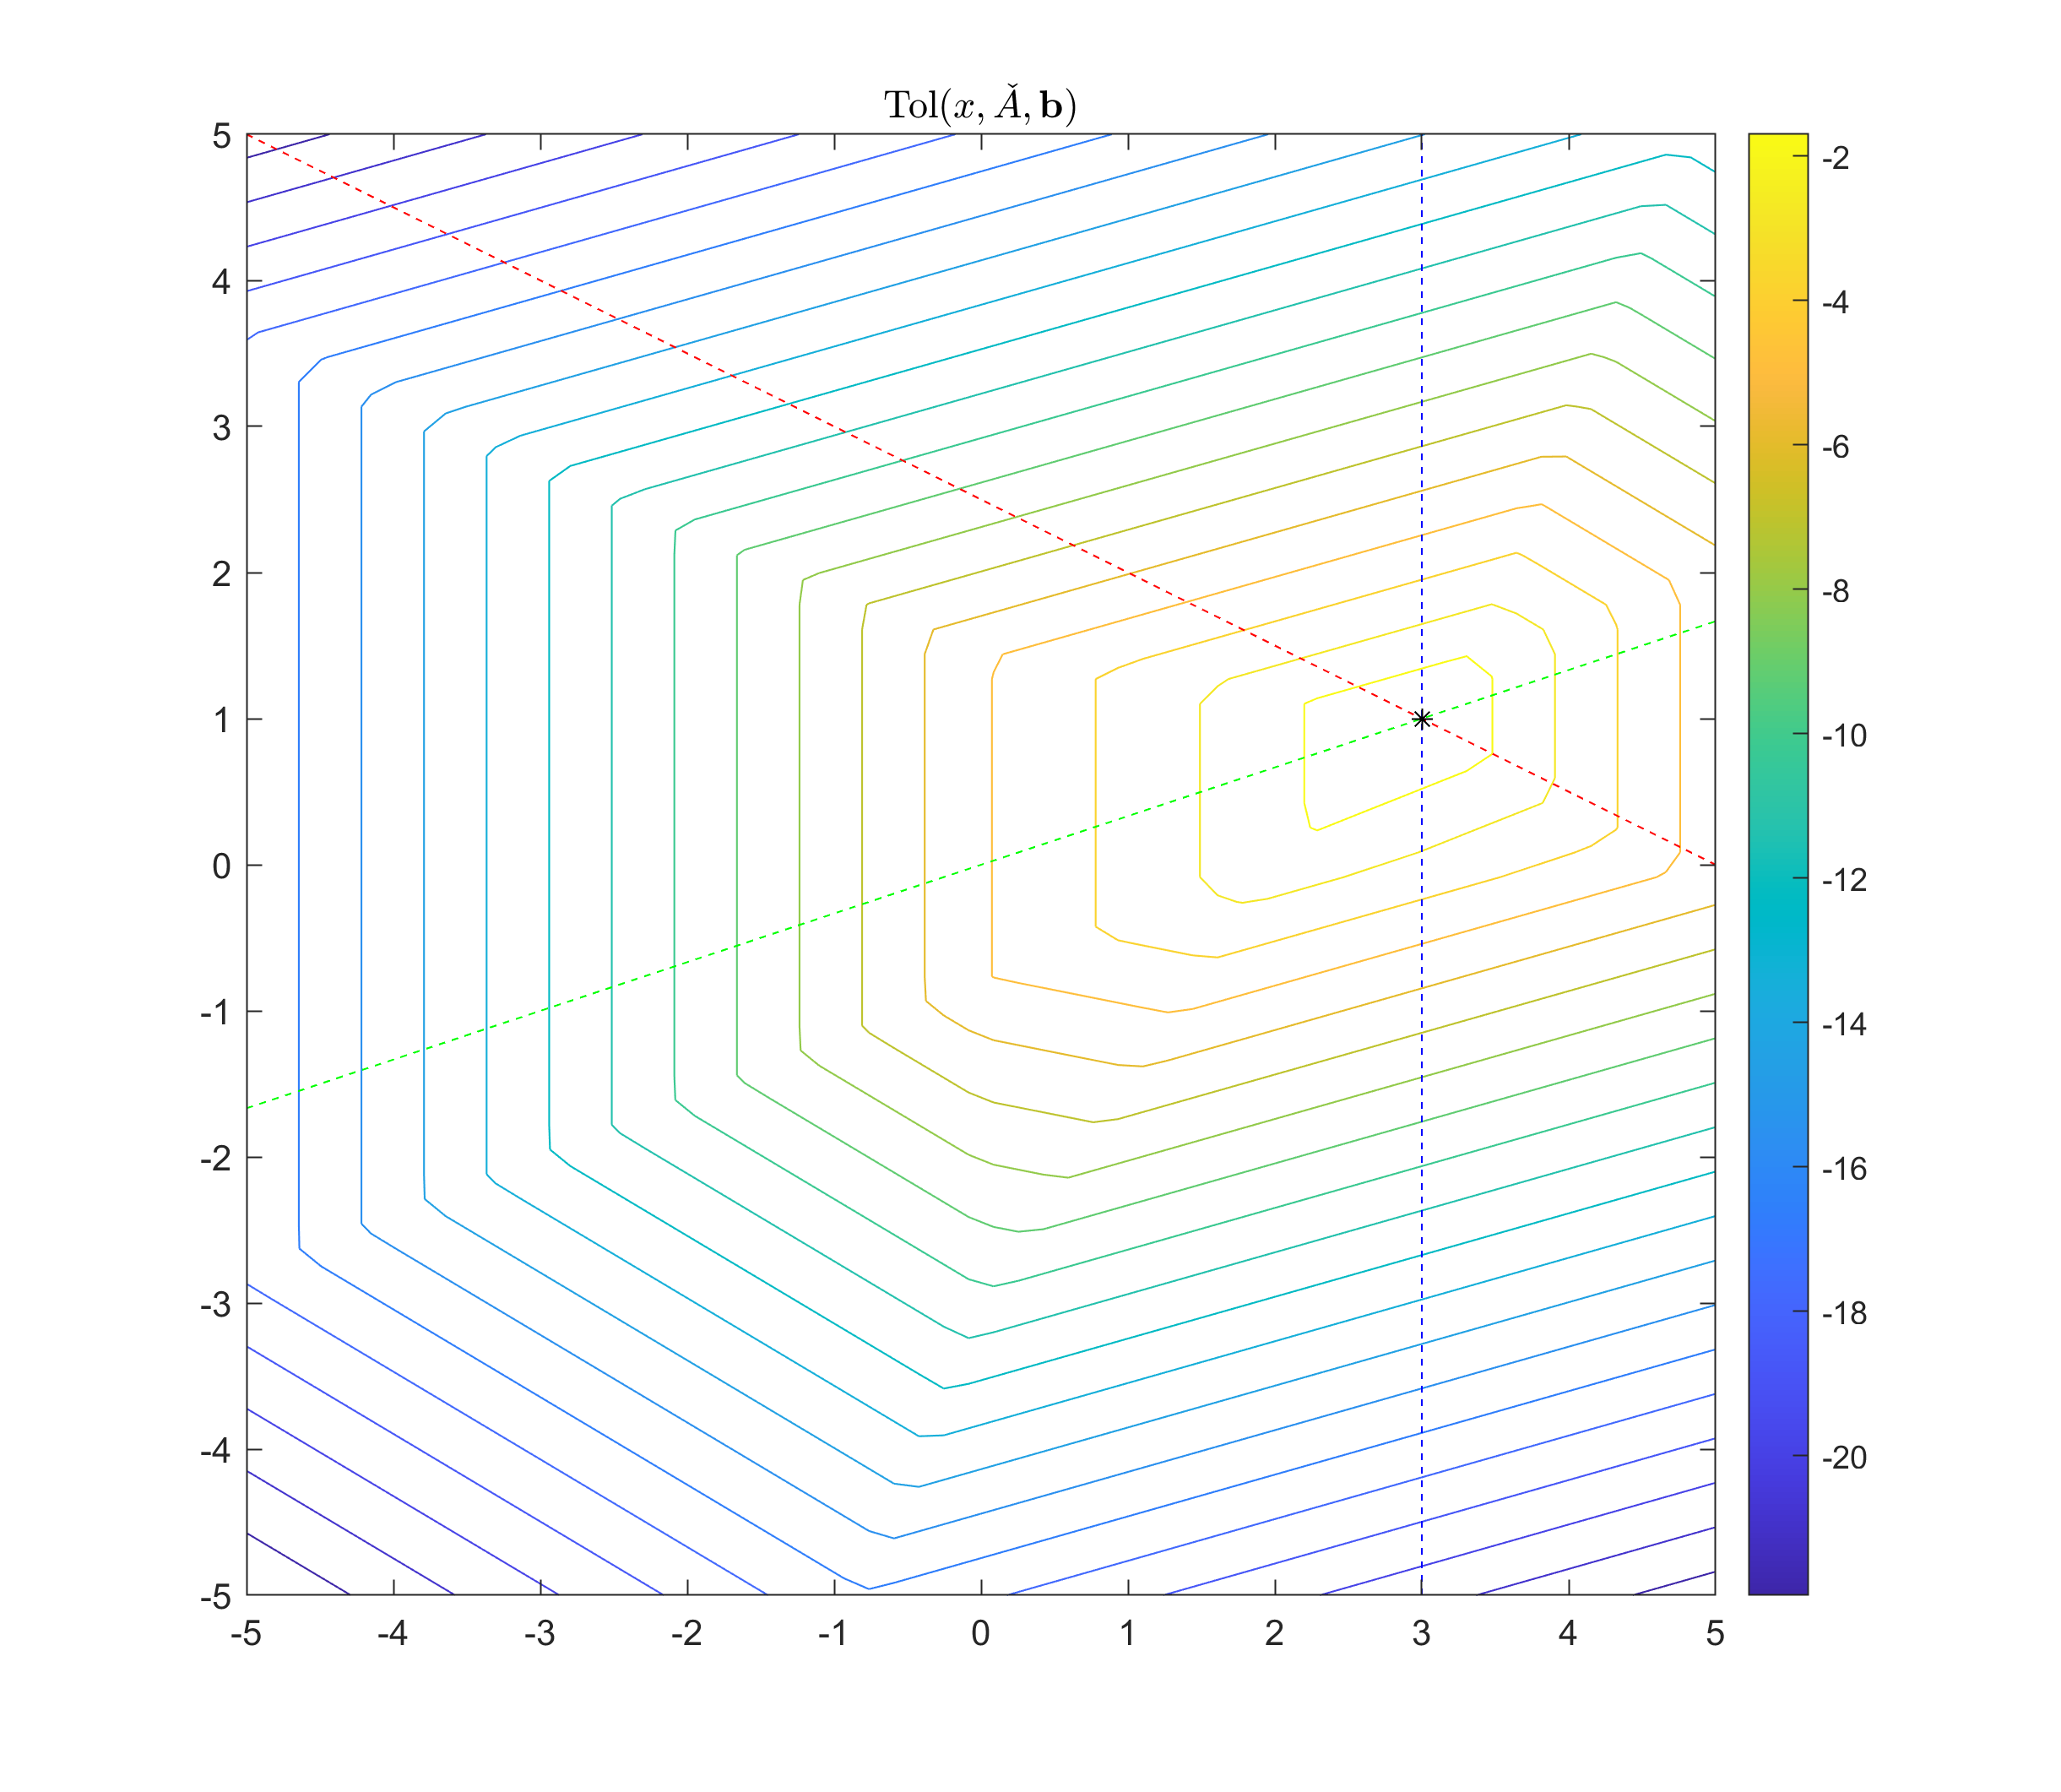
\includegraphics[width=15cm]{img/linesEye.png}
    \caption{График $\mathrm{Tol}(x,\check{\mbf{A}},\mbf{b})$ с корректировкой матрицы в целом}
    \label{fig:linesEye}
\end{figure}
Результат корректировки первой строки:
\begin{equation*}
    \check{\mbf{A}}=\begin{pmatrix}
    1&2\\
    1&[-4,\:-2]\\
    [1,\:3]&0
    \end{pmatrix},\;\mathrm{arg}\max\mathrm{Tol}(x,\check{\mbf{A}}, \mbf{b})=(3,1)
\end{equation*}
\begin{figure}[H]
    \centering
    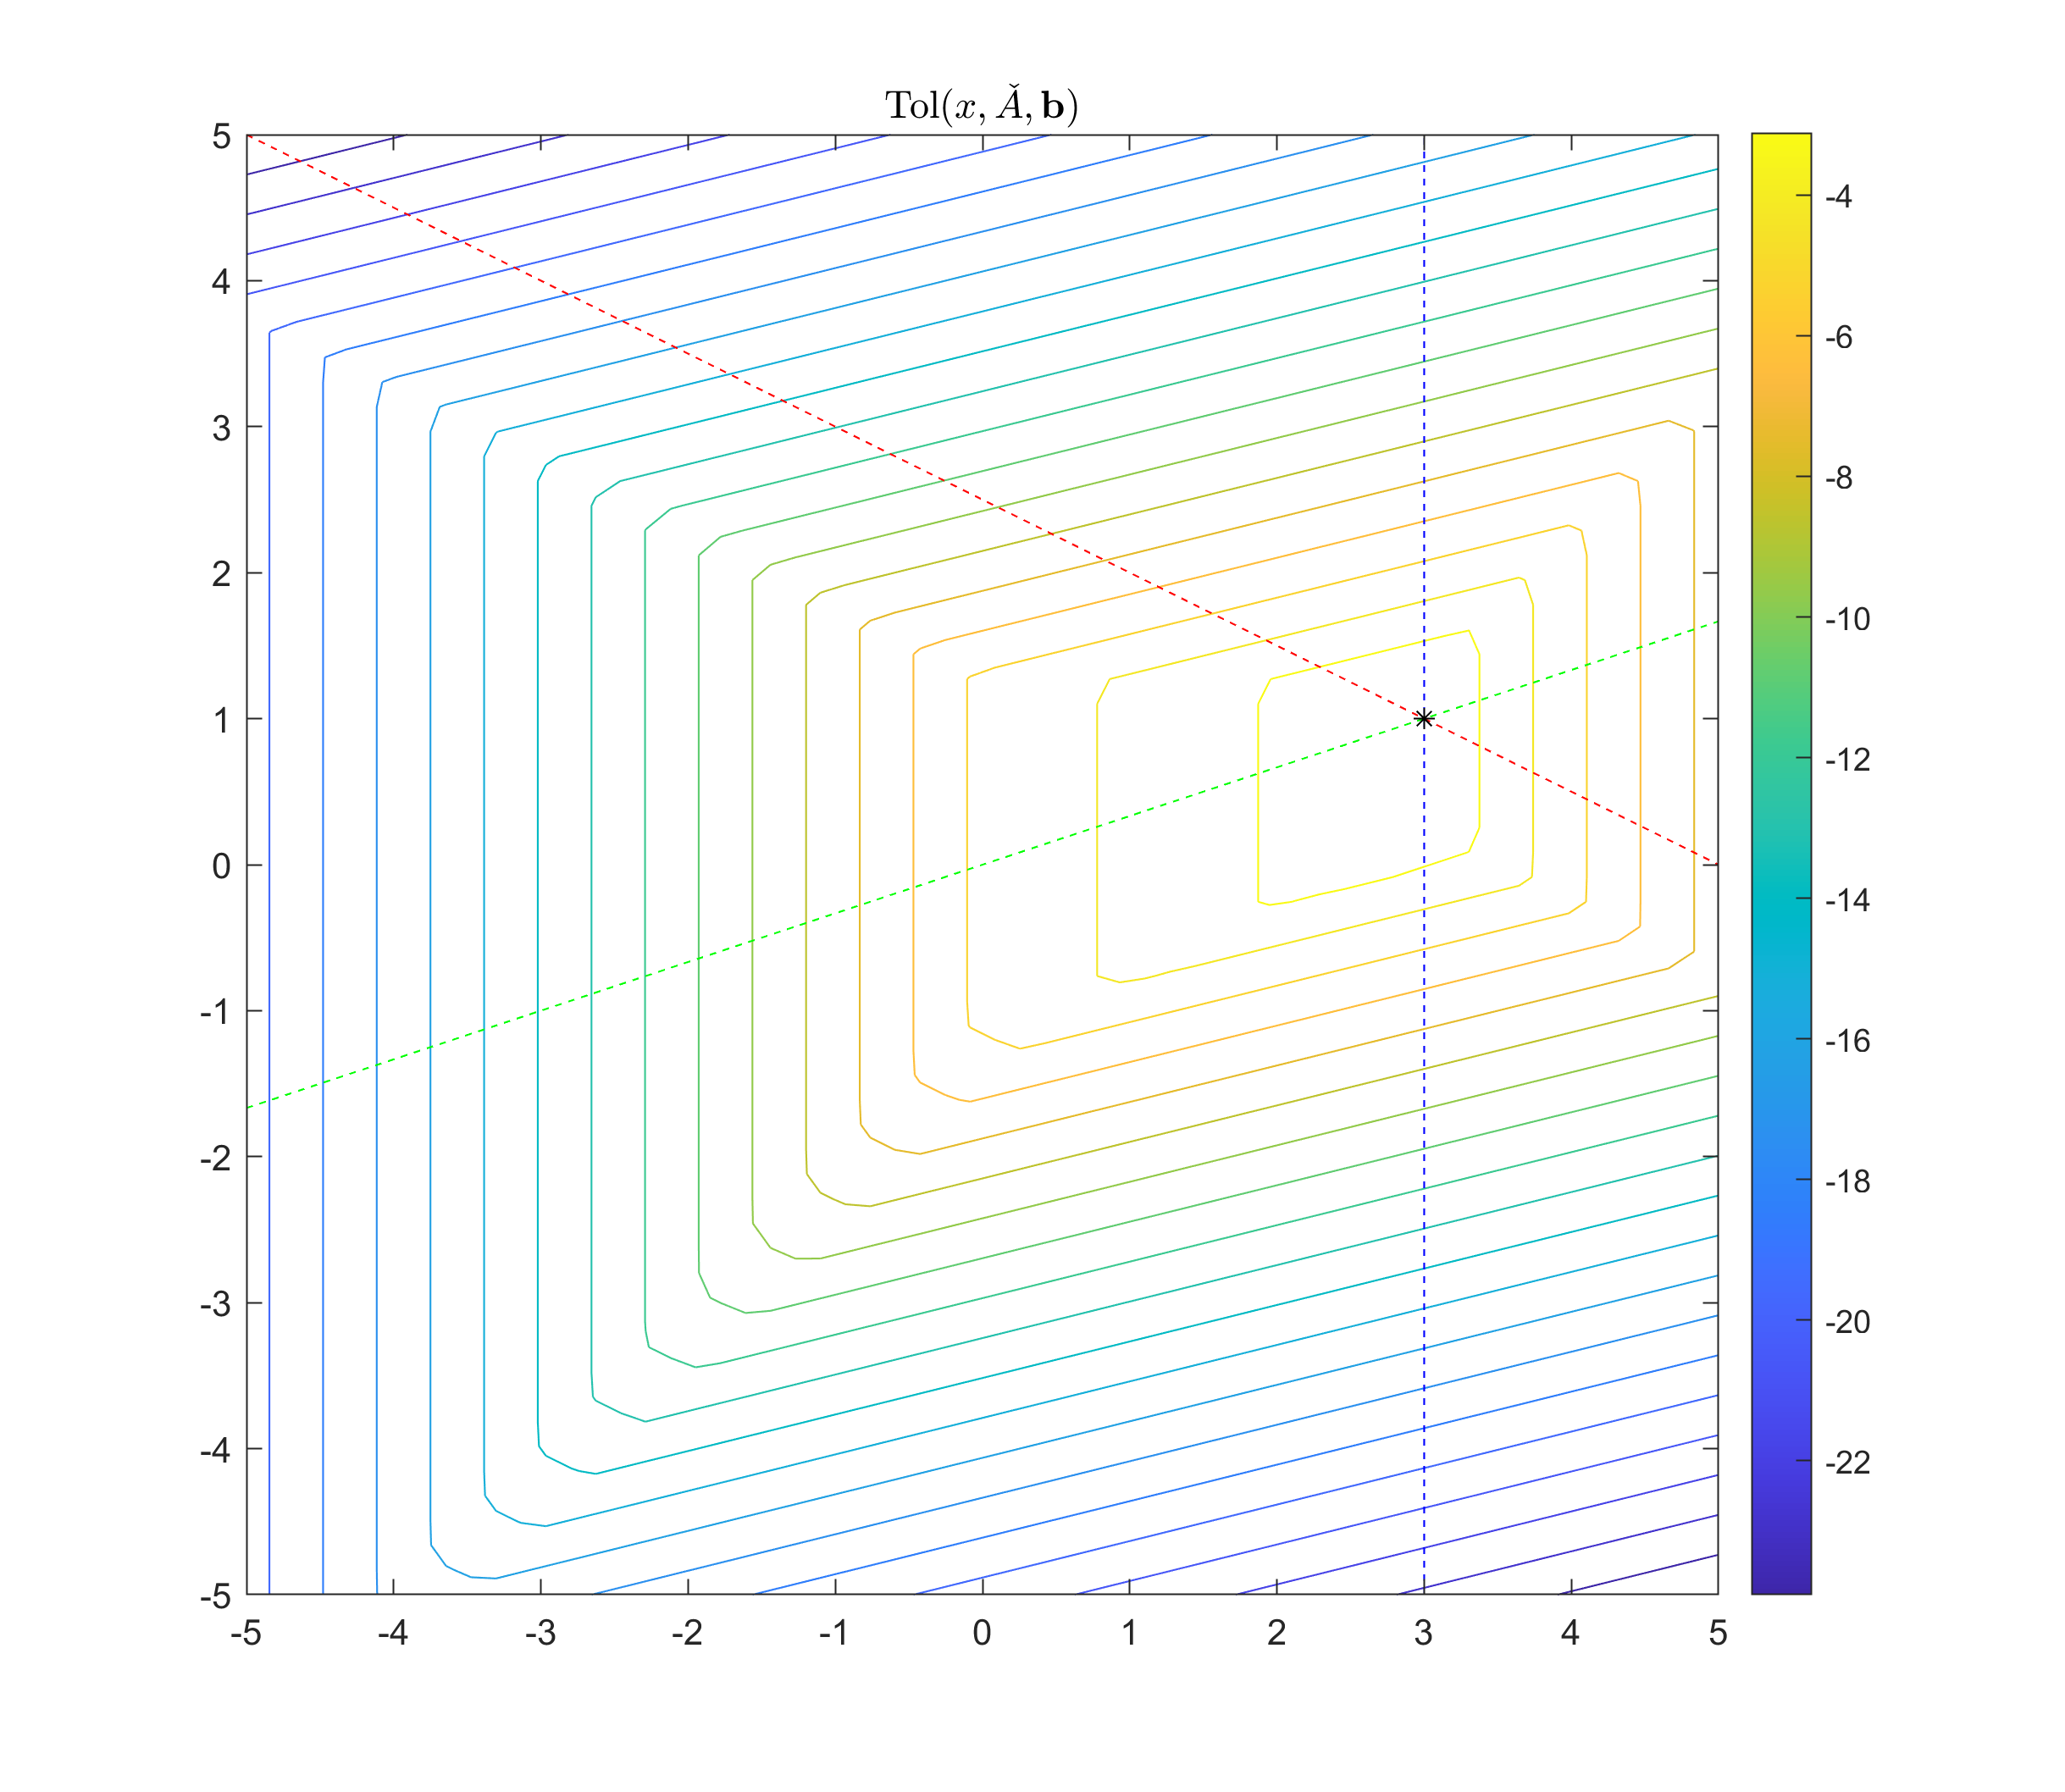
\includegraphics[width=15cm]{img/lines1.png}
    \caption{График $\mathrm{Tol}(x,\check{\mbf{A}},\mbf{b})$ с корректировкой первой строки матрицы}
    \label{fig:lines1}
\end{figure}
Результат корректировки второй строки:
\begin{equation*}
    \check{\mbf{A}}=\begin{pmatrix}
    [0,\:2]&[1,\:3]\\
    1&-3\\
    [1,\:3]&0
    \end{pmatrix},\;\mathrm{arg}\max\mathrm{Tol}(x,\check{\mbf{A}}, \mbf{b})=(3,1)
\end{equation*}
\begin{figure}[H]
    \centering
    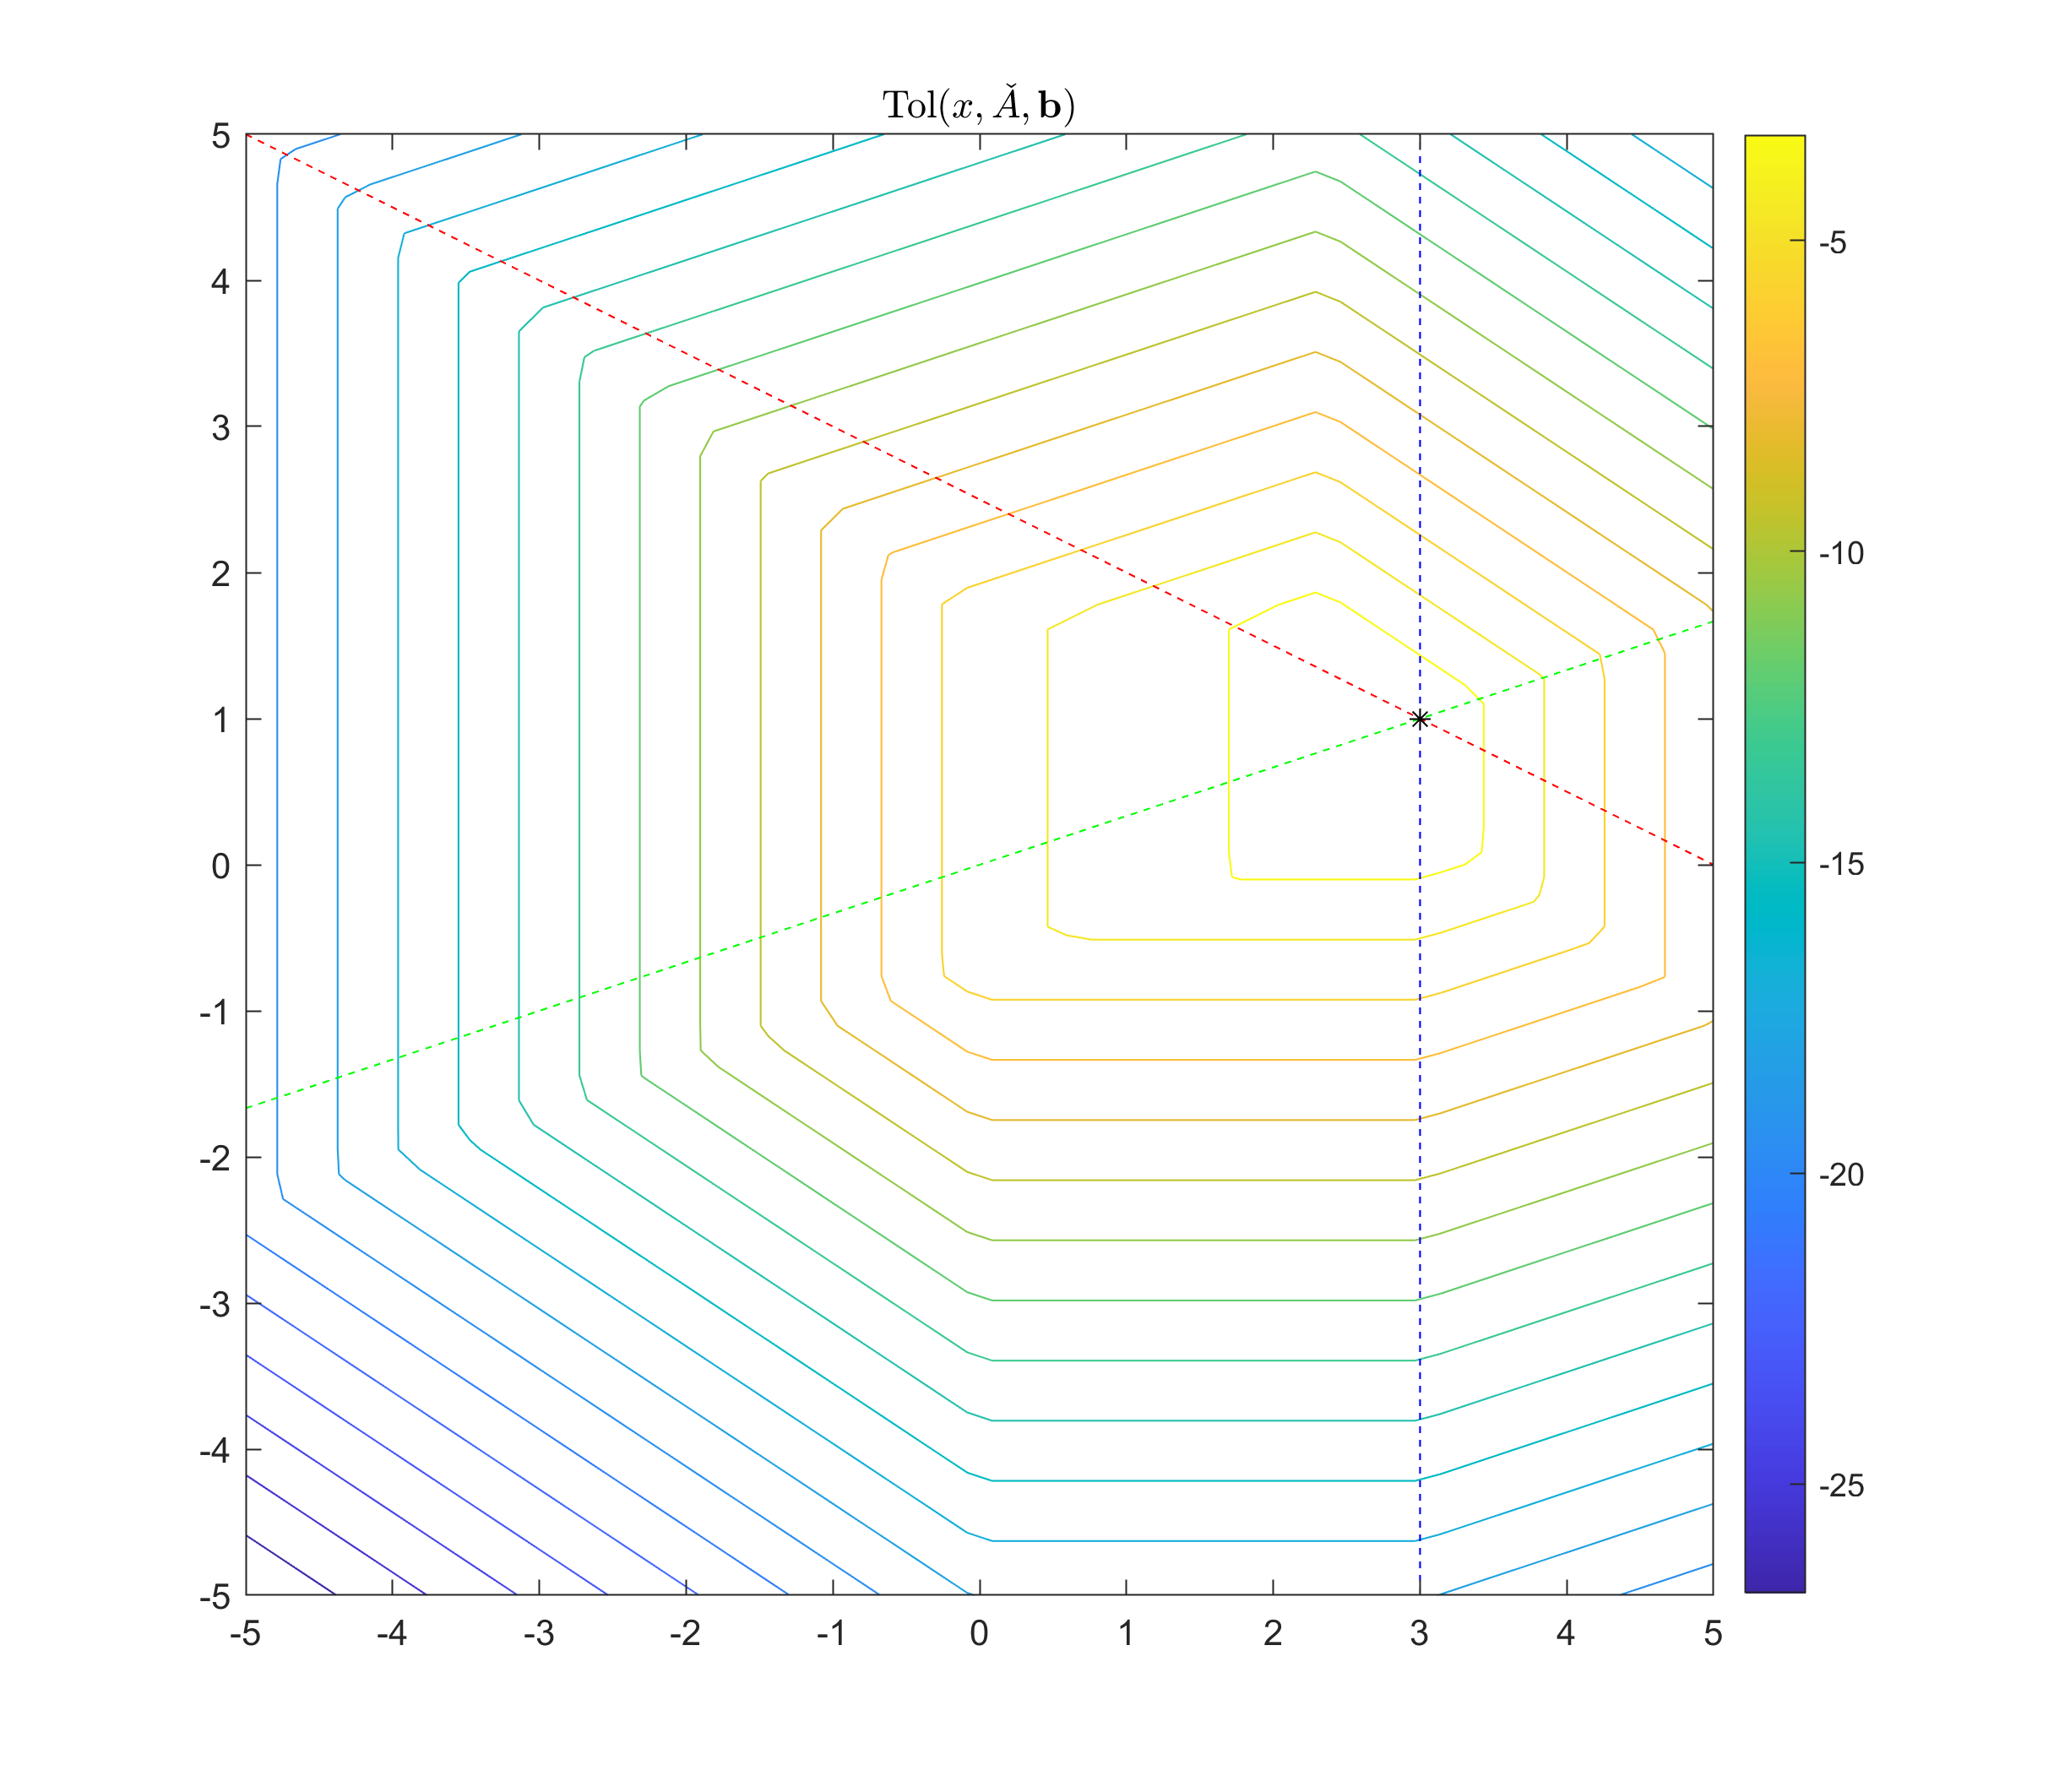
\includegraphics[width=15cm]{img/lines2.png}
    \caption{График $\mathrm{Tol}(x,\check{\mbf{A}},\mbf{b})$ с корректировкой второй строки матрицы}
    \label{fig:lines2}
\end{figure}
Результат корректировки третьей строки:
\begin{equation*}
    \check{\mbf{A}}=\begin{pmatrix}
    [0,\:2]&[1,\:3]\\
    1&[-4,\:-2]\\
    2&0
    \end{pmatrix},\;\mathrm{arg}\max\mathrm{Tol}(x,\check{\mbf{A}}, \mbf{b})=(2.71,1.14)
\end{equation*}
\begin{figure}[H]
    \centering
    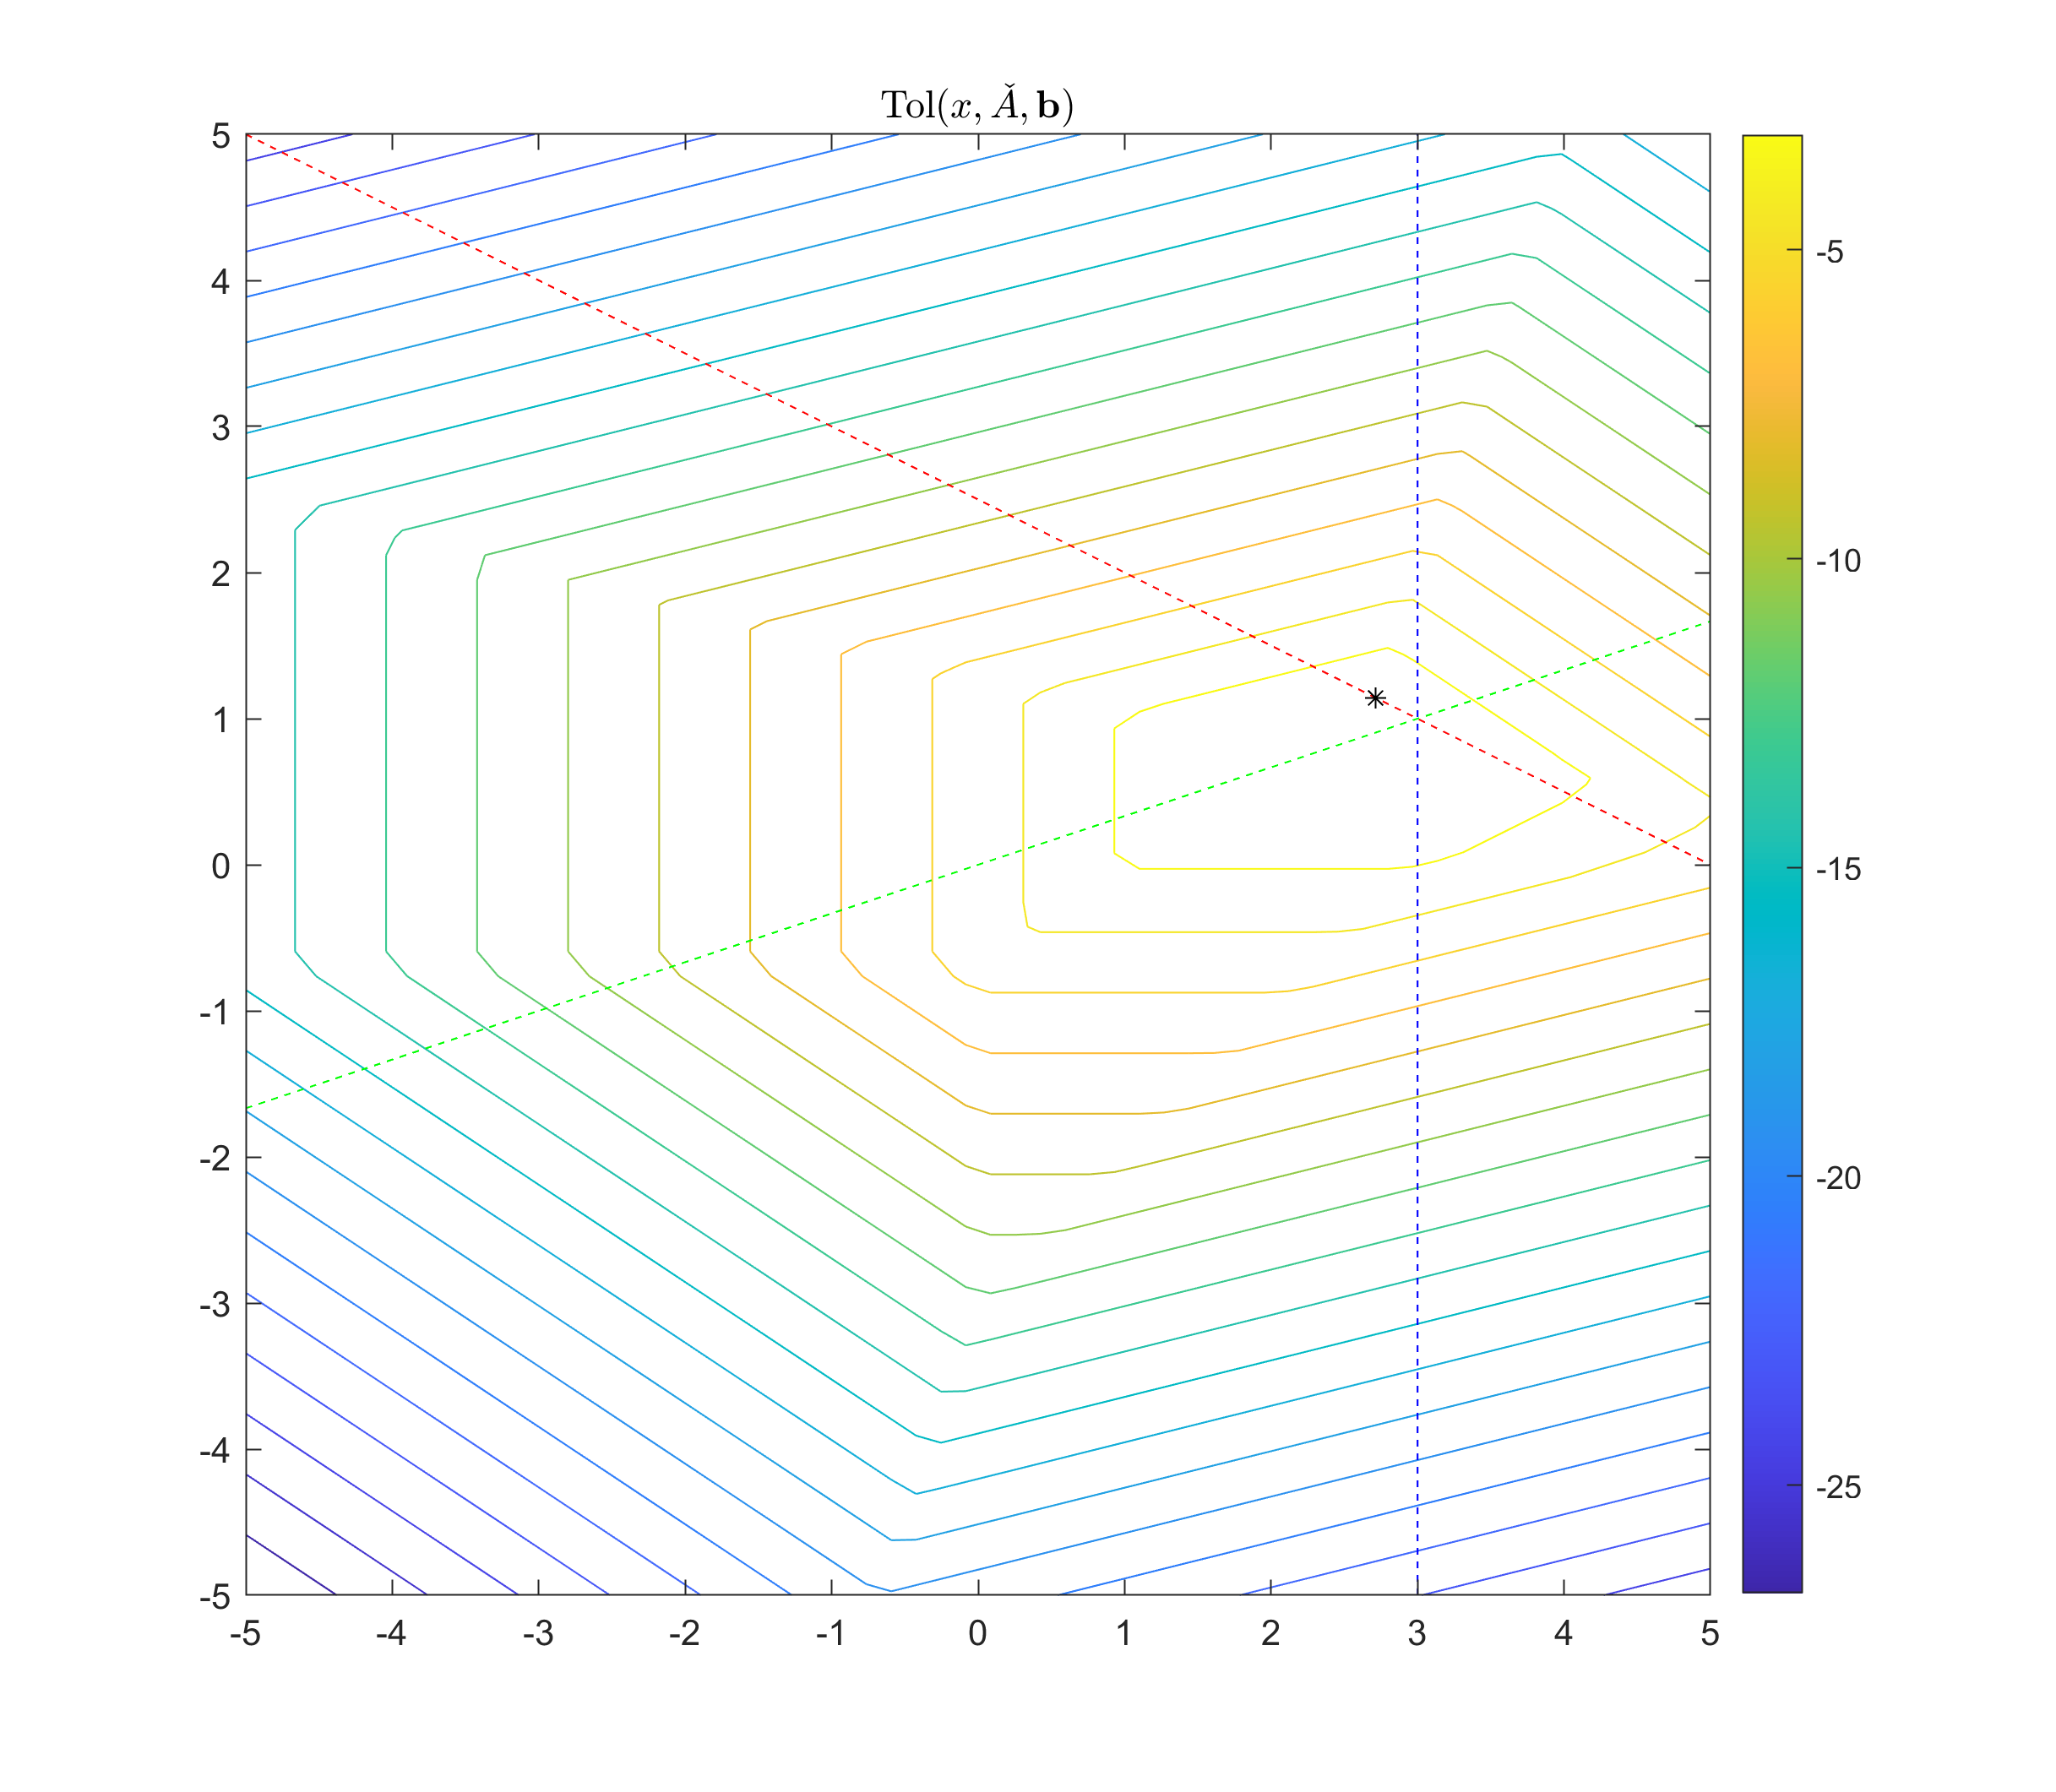
\includegraphics[width=15cm]{img/lines3.png}
    \caption{График $\mathrm{Tol}(x,\check{\mbf{A}},\mbf{b})$ с корректировкой третьей строки матрицы}
    \label{fig:lines3}
\end{figure}
\section{Обсуждение}
\begin{enumerate}
    \item Коррекция правой части с коэффициентом расширения $K$ влечет увеличение значения максимума распознающего функционала на $K$.
    \item Коррекция правой части не меняет форму распознающего функционала, не меняет положение максимума.
    \item Исходя из результатов графика \ref{fig:biverve}, можно заключить, что с помощью $\mathrm{ive}$ и $\mathrm{rve}$ можно оценить $\Xi_{\mathrm{tol}}$. На данном графике квадрат с центром в точке максимума $\mathrm{Tol}(x)$ и стороной $2\cdot\mathrm{ive}\:(\mbf{A}, \hat{\mbf{b}})$ дает внутреннюю оценку допускового множества, аналогичный квадрат со стороной $2\cdot\mathrm{rve}\:(\mbf{A}, \hat{\mbf{b}})$ - внешнюю. Обе оценки довольно точные. Вероятно, рассматриваемые числовые характеристики пригодны для оценки $\Xi_{\mathrm{tol}}$ в многомерных случаях, когда затруднительно найти нулевую границу распознающего функционала.
    \item Коррекция матрицы ИСЛАУ меняет форму распознающего функционала во всех рассмотренных преобразованиях. 
    \item При достижении разрешимости ИСЛАУ за счет коррекции матрицы получен отрезок, на котором достигается максимальное значение распознающего функционала, равное 0. Увеличить значение максимума или расширить область $\Xi_{\mathrm{tol}}$ не получилось предположительно из-за вида второго уравнения ИСЛАУ: только одна интервальная величина на две точечные.
    \item При вырождении $\Xi_{\mathrm{tol}}$ по хотя бы одной координате оценки вариабельности становятся равны 0.
    \item Не во всех случаях изменение матрицы влияет на положение максимума распознающего функционала. Из четырех рассмотренных ситуаций смещение точки максимума произошло только при правке третьей строки матрицы: смещение произошло вдоль прямой, образованной первой строкой СЛАУ $\imid{(\mbf{A})}x=\imid{\mbf{b}}$. Предположительно такая ситуация возникла ввиду пересечения всех трех прямых в одной точке $(3,1)$.
\end{enumerate}
\section*{Исходный код}
С исходным кодом программы и отчета можно ознакомиться в репозитории \url{https://github.com/Stasychbr/IntervalArith}.
\end{document}
